\documentclass[a4paper,10pt]{article}
\usepackage[utf8]{inputenc}

% ----  Useful packages % ---- 
\usepackage{amsmath}
\usepackage{graphicx}
\usepackage{amsfonts}
\usepackage{amsthm}
\usepackage{amssymb}
\usepackage{mathtools}
\usepackage{enumitem}
% ----  Useful packages % ---- 

\usepackage{wrapfig}
\usepackage{caption}
\usepackage{subcaption}
\usepackage{hyperref}
\hypersetup{
    colorlinks,
    citecolor=black,
    filecolor=black,
    linkcolor=black,
    urlcolor=black
}

\graphicspath{ {./images/} }

% ---- Set page size and margins replace ------
\usepackage[letterpaper,top=2cm,bottom=2cm,left=3cm,right=3cm,marginparwidth=1.75cm]{geometry}
% ---- Set page size and margins replace ------

% ------- NOTA ------
\theoremstyle{remark}
\newtheorem{note}{Note}[subsection]
% ------- NOTA ------

% ------- OSSERVAZIONE ------
\theoremstyle{definition}
\newtheorem{observation}{Osservazione}[subsection]
% ------- OSSERVAZIONE ------

% ------- DEFINIZIONE ------
\theoremstyle{plain}
\newtheorem{definition}{Definizione}[subsection]
% ------- DEFINIZIONE ------

% ------- ESEMPIO ------
\theoremstyle{definition}
\newtheorem{example}{Esempio}[subsection]
% ------- ESEMPIO ------

% ------- DIMOSTRAZIONE ------
\theoremstyle{definition}
\newtheorem{demostration}{Dimostrazione}[subsection]
% ------- DIMOSTRAZIONE ------

% ------- TEOREMA ------
\theoremstyle{definition}
\newtheorem{theorem}{Teorema}[subsection]
% ------- TEOREMA ------

% ------- COROLLARIO ------
\theoremstyle{plain}
\newtheorem{corollaries}{Corollario}[theorem]
% ------- COROLLARIO ------

% ------- PROPOSIZIONE ------
\theoremstyle{plain}
\newtheorem{proposition}{Proposizione}[subsection]
% ------- PROPOSIZIONE ------

% ---- Footer and header ---- 
\usepackage{fancyhdr}
\pagestyle{fancy}
\fancyhf{}
\fancyhead[LE,RO]{A.A 2021-2022}
\fancyhead[RE,LO]{Algebra Lineare}
\fancyfoot[RE,LO]{\rightmark}
\fancyfoot[LE,RO]{\thepage}

\renewcommand{\headrulewidth}{.5pt}
\renewcommand{\footrulewidth}{.5pt}
% ---- Footer and header ---- 

% ----  Language setting ---- 
\usepackage[italian, english]{babel}
% ----  Language setting ---- 

\title{\textbf{Algebra Lineare}}
\author{Realizzato da: Giuntoni Matteo}
\date{A.A. 2021-2022}

\begin{document}
\begin{titlepage} %crea l'enviroment
	\begin{figure}[t] %inserisce le figure
		\centering
\includegraphics[width=0.98\textwidth]{marchio_unipi_pant541.png}
	\end{figure}
	\vspace{20mm}
	
	\begin{Large}
		\begin{center}
			\textbf{Dipartimento di Informatica\\ Corso di Laurea Triennale in Informatica\\}
			\vspace{20mm}
			{\LARGE{Corso a Libera Scelta - 6 CFU}}\\
			\vspace{10mm}
			{\huge{\bf Computer Graphics}}\\
		\end{center}
	\end{Large}
	
	
	\vspace{36mm}
	%minipage divide la pagina in due sezioni settabili
	\begin{minipage}[t]{0.47\textwidth}
		{\large{\bf Professore:}\\ \large{Prof. }}
	\end{minipage}
	\hfill
	\begin{minipage}[t]{0.47\textwidth}\raggedleft
		{\large{\bf Autore:}\\ \large{Filippo Ghirardini}}
	\end{minipage}
	
	\vspace{25mm}
	
	\hrulefill
	
	\vspace{5mm}
	
	\centering{\large{\bf Anno Accademico 2023/2024 }}
	
\end{titlepage}
\tableofcontents
\newpage
\maketitle
\begin{center}
    \vspace{-20pt}
    \rule{11cm}{.1pt} 
\end{center}
\section{Introduzione}

\subsection{Insiemi Numerici}
Un insieme di numeri è una raccolta di elementi. Alcuni degli insiemi che verranno utilizzati maggiormente in questo corso sono:
\begin{itemize}
    \item \textbf{N. Naturali} cioè tutti gli interi non negativi: $\mathbb{N}$ = $\{0, 1, 2, 3, 4, ...\}$.
    \item \textbf{N. Interi} cioè tutti gli interi con segno qualsiasi: $\mathbb{Z} = \{..., -3, -2, -1, 0, 1, 2, 3, ...\}$.
    \item \textbf{N. Razionali}, cioè le frazioni: $\mathbb{Q} = \{\frac{p}{q}$ dove p e q $\in \mathbb{Z}$ e $q \neq 0\}$. \\
    Un sottoinsieme sono le \textbf{classi di equivalenza} che sono tutte le frazioni semplificate ai minimi termini. 
    \item \textbf{N. Reali}, che possono essere visti come tutti gli elementi rappresentabili su una retta: $\mathbb{R}$ 
\end{itemize}
\begin{note}
I vari insiemi si contengono fra di loro. ($\mathbb{N} \subset \mathbb{X} \subset \mathbb{Q} \subset \mathbb{R}$) 
\end{note}
\begin{note}
Esistono molti numeri reali che non sono razionali e non si possono scrivere come frazioni. E.g. $\sqrt{2}, \pi, ...$
\end{note}

\subsection{Intervalli}
\begin{definition}[Intervallo]
    Un sottoinsieme $I \subseteq \mathbb{R}$ è un intervallo se $\forall \: x,\:y \in I$ $\mid$ $x < y$ $\wedge$ $\forall z \mid x < z < y$ ho che $z \in I$. [\ref{fig:intervallo}]
\end{definition}
\begin{wrapfigure}{l}{7cm}
	\vspace{-20pt}
	\centering
	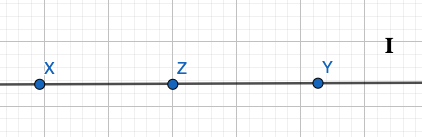
\includegraphics[width=5cm]{Intervallo.png}
	\caption{Tutto il segmento fra x e y deve stare in I}
	\label{fig:intervallo}
\end{wrapfigure}
I è un intervallo se ogni \emph{ogni} punto che prendo tra gli estremi dell'intervallo, questo appartiene all'intervallo stesso.
\\\\\\\\\\
\begin{example}
Esempi di intervalli.\\ \\
Questo caso \textbf{è un intervallo} \hspace{3.2cm} Questo caso \textbf{non è un intervallo} fra A e D.
\begin{figure}[h!]
    \vspace{-10pt}
    \begin{subfigure}{.5\textwidth}
        \hspace{-50pt}
        \centering
        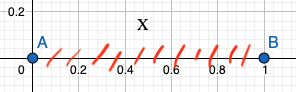
\includegraphics[width=6cm]{Esempio-intervallo-1.png}
        \caption{$A = \{x \in \mathbb{R} \: | \: 0<x<1\}$}
    \end{subfigure}
    \begin{subfigure}{.5\textwidth}
        \centering
        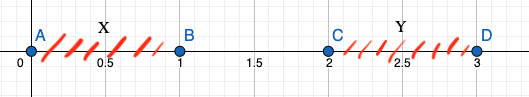
\includegraphics[width=7.5cm]{Esempio-intervallo-2.png}
        \caption{$C = \{x \in \mathbb{R} \: | \: 0<x<1 \: \vee \: z<x<3\}$}
    \end{subfigure}
\end{figure}
\end{example}

\newpage
\subsection{Notazione}
Con $a, b \in \mathbb{R}$ e con $a < b$ è possibile scrivere le notazioni in tabella \ref{tab:notazione-intervalli}.
\begin{table}[h!]
    \centering
    \setlength{\tabcolsep}{7pt}
    \renewcommand{\arraystretch}{2}
    \begin{tabular}{|c|c|c|} \hline
        [a, b] & Intervallo chiuso di estremi a e b & $\{x \in \mathbb{R} \: | \: a \leq x \leq b\}$ \\ \hline
        (a, b) & Intervallo aperto & $\{x \in \mathbb{R} \: | \: a < x < b\}$ \\ \hline
        [a, b) & Intervallo semi aperto a destra & $\{x \in \mathbb{R} \: | \: a \leq x < b\}$ \\ \hline
        (a, b] & Intervallo semi aperto a sinistra & $\{x \in \mathbb{R} \: | \: a < x \leq b\}$ \\ \hline
        [a, $+\infty$) & Semiretta chiusa a sinistra & $\{x \in \mathbb{R} \: | \: a \leq x\}$ \\ \hline
        ($-\infty$, b] & Semiretta chiusa a destra & $\{x \in \mathbb{R} \: | \: x \leq b\}$ \\ \hline
        ($-\infty$, $+\infty$) & Insieme di tutti i numeri $\mathbb{R}$ & $\{x \in \mathbb{R}\}$ \\ \hline
    \end{tabular}
    \caption{Notazione Intervalli}
    \label{tab:notazione-intervalli}
\end{table}
% !TeX spellcheck = it_IT
\newpage
\section{Algoritmo di Gauss}
Utilizzando le proprietà (1), (2) e (3) viste sopra si ottiene un algoritmo per semplificare $(E)$.
In un primo momento si considera $b_1 = \ldots = b_n = 0$ e mettiamo i coefficienti in una matrice $n \times m$, [$a_{ij}$]:
\[
\begin{bmatrix}
a_{11} & a_{12} & \ldots & a_{1m}\\
a_{21} & a_{22} & \ldots & a_{2m}\\
& \vdots & & \\
a_{n1} & a_{n2} & \ldots & a_{nm}
\end{bmatrix}
\xRightarrow[]{\text{(Con operazioni)}}
\begin{bmatrix}
\ldots \\
a_{j1} + \lambda a_{i1} + a_{j2} + \lambda a_{i2} + \ldots + a_{jm} + \lambda a_{im}\\
\ldots
\end{bmatrix}
\]
Le operazioni di prima si traducono come:
\begin{enumerate}
    \item Scambiare due righe fra di loro.
    \item Sostituire la riga $R_j$ con la riga $R_j + \lambda R_i$.
    \item Moltiplicare una riga per $\lambda \neq 0$.
\end{enumerate}
Partendo da una matrice l'algoritmo produce, utilizzando le 2 operazioni una matrice detta \textbf{a forma di scalini}.

\begin{definition}[Matrice a forma a scalini]
Una matrice è a forma a scalini (per righe) se:
\begin{itemize}
    \item Le righe $(0,\ldots,0)$ sono "in fondo" alla matrice (partendo da sinistra).
    \item Il primo elemento di ogni riga (se esiste) è a destra del primo elemento diverso da 0 della riga precedente. Tale elemento si dice pivot.
\end{itemize}
\end{definition}

\begin{definition}[Pivot]
Il primo elemento diverso a 0 d ogni riga di una matrice (nella forma a scalini) si chiama pivot.
\end{definition}

\begin{example}
Esempio di matrici in forma a scalini e non:
\vspace{-10pt}
\begin{figure}[h!]
    \centering
    \begin{minipage}{.3\linewidth}
        \centering
        \[
            \begin{bmatrix}
            1 & 1 & 1\\
            1 & 1 & 0\\
            0 & 0 & 1
            \end{bmatrix}
        \]
        NO
    \end{minipage}
    \begin{minipage}{.3\linewidth}
        \centering
        \[
            \begin{bmatrix}
            1 & 1 & 1\\
            0 & 1 & 1\\
            0 & 0 & 1
            \end{bmatrix}
        \]
        SI
    \end{minipage}
    \begin{minipage}{.3\linewidth}
        \centering
        \[
            \begin{bmatrix}
            0 & 1 & 1\\
            1 & 1 & 0\\
            0 & 0 & 1
            \end{bmatrix}
        \]
        NO
     \end{minipage}
\end{figure}
\end{example}

\begin{definition}[Algoritmo di Gauss]
Ogni matrice $n \times m$ si mette in forma a scalini (per righe) con operazioni del tipo (A) e (B).
\begin{enumerate}
    \item Se la matrice è già in forma a scalini abbiamo finito.
    \item Si cerca il primo elemento diverso da 0 della prima colonna diversa da 0.
    \item Cambiamo righe si può supporre che questo elemento è il pivot della prima riga. Notiamo che se siamo in forma a scalini abbiamo finito sennò procediamo.
    \item Si annullano tutti gli elementi della colonna del pivot sotto il pivot  con operazioni del tipo (B). Se siamo in forma a scalini finiamo sennò continuiamo.
    \item Non consideriamo la prima riga (la cancelliamo) e ricominciamo con l'algoritmo.
\end{enumerate}
\end{definition}

\newpage
\begin{example}
Prendiamo il seguente sistema di equazioni e scriviamolo su una matrice:
\[
\begin{array}{l}
x_1 + x_2 + 3x_4 = 0\\
3x_1 - x_2 + x_3 + 10x_4 = 0\\
x_1 + 5x_2 + 2x_3 + x_4 = 0
\end{array}
\hspace{.2cm}
\Rightarrow
\hspace{.2cm}
\begin{bmatrix}
1 & -1 & 0 & 3\\
3 & -1 & 1 & 10\\
1 & 5 & 2 & 1
\end{bmatrix}
\:\:
\parbox{4cm}{Da qui iniziamo ad applicare l'algoritmo}
\]
\end{example}
\begin{figure}[h!]
    \vspace{-20pt}
    \centering
    \begin{minipage}{.3\linewidth}
        \centering
        \[
            \begin{bmatrix}
            \underline{1} & -1 & 0 & 3\\
            3 & -1 & 1 & 10\\
            1 & 5 & 2 & 1
            \end{bmatrix}
        \]
        Applichiamo il passo (1) e troviamo 1 come pivot
    \end{minipage}
    \begin{minipage}{.3\linewidth}
        \centering
        \[
            \begin{bmatrix}
            1 & -1 & 0 & 3\\
            0 & 3 & 1 & 1\\
            0 & 6 & 2 & -1
            \end{bmatrix}
        \]
        Applichiamo il passo (3) e calcoliamo $R_2 = R_2 - 3R_1$ e $R_3 = R_3 - R_1$
    \end{minipage}
    \begin{minipage}{.3\linewidth}
        \centering
        \[
            \begin{bmatrix}
            0 & 3 & 1 & 1\\
            0 & 0 & -1 & -5
            \end{bmatrix}
        \]
        Applichiamo (4) e non consideriamo la riga $R_1$ per poi ripetere l'operazione (3) facendo $R_3 = R_3 - 3R_2$
    \end{minipage}
\end{figure}
\hspace{-15pt}Vediamo così che la matrice finale è ha forma di scalini. Possiamo ora prendendo i numeri nella matrice andare a riscrivere il sistema di equazioni associato. Il sistema è il seguente:
\[
\begin{array}{l}
x_1 + x_2 + 3x_4 = 0\\
2x_2 + x_3 + x_4 = 0\\
-x_3 + 5x_4 = 0
\end{array}
\hspace{.2cm}
\xRightarrow[]{\text{(E la matrice)}}
\hspace{.2cm}
\begin{bmatrix}
1 & -1 & 0 & 3\\
0 & 3 & 1 & 1\\
0 & 0 & -1 & -5
\end{bmatrix}
\]
A questo punto se consideriamo $x_4 = t$ abbiamo che $x_3 = -5t$ e di conseguenza $2x_2 - 5t + t = 0$ e quindi $x_2 = 2t$ ed ancora abbiamo $x_1 = 2t -3t -t$. Possiamo dunque dire che in questo esempio $x_4$ essendo una colonna senza pivot è una "variabile libera" e quindi ci sono più soluzioni.\\
Potrebbe esserci anche il caso in cui la colonna contenga un pivot e quinci ci sarebbe un unica soluzione.\\\\
Se consideriamo invece un sistema non omogeneo formato aggiungendo una colonna con $b_1, ..., b_n$, è possibile utilizzare ugualmente l'algoritmo di guass aggiungendo una colonna alla matrice.

\begin{example}
Prendiamo il seguente sistema di equazioni e mettiamolo su una matrice:
\end{example}
\begin{figure}[h!]
    \vspace{-20pt}
    \centering
    \begin{minipage}{1\linewidth}
        \centering
        \[
            \begin{array}{l}
            x_1 + x_2 + x_3 + 2x_4 = 9\\
            x_1 + x_2 + 2x_3 + x_4 = 8\\
            x_1 + 2x_2 + x_3 + x_4 = 7\\
            2x_1 + x_2 + x_3 + x_4 = 6
            \end{array}
            \hspace{.2cm}
            \Rightarrow
            \hspace{.2cm}
            \begin{bmatrix}
            1 & 1 & 1 & 2 & 9\\
            1 & 1 & 2 & 1 & 8\\
            1 & 2 & 1 & 1 & 7\\
            2 & 1 & 1 & 1 & 6
            \end{bmatrix}
            \xRightarrow[]{\text{Uso algoritmo}}
            \begin{bmatrix}
            1 & 1 & 1 & 2 & 9\\
            1 & 1 & 2 & 1 & 8\\
            1 & 2 & 1 & 1 & 7\\
            2 & 1 & 1 & 1 & 6
            \end{bmatrix}
            \begin{array}{r}
            R_2 = R_2 - R_1\\
            R_3 = R_3 - R_1\\
            R_4 = R_4 - 2R_1
            \end{array}
        \]
        Il pivot è in $R_1$ ed è 1, da qui applichiamo (3) e poi (4).
    \end{minipage}
\end{figure}
\vspace{-15pt}
\begin{figure}[h!]
    \begin{minipage}{1\linewidth}
        \centering
        \[
            \begin{bmatrix}
            0 & 0 & 1 & 2 & -1\\
            0 & 1 & 0 & -1 & -2\\
            0 & -1 & -1 & -3 & -12
            \end{bmatrix}
            \Rightarrow
            \begin{bmatrix}
            0 & 1 & 0 & -1 & -2\\
            0 & 0 & 1 & -1 & -1\\
            0 & -1 & -1 & -3 & -12
            \end{bmatrix}
            \Rightarrow
            \begin{bmatrix}
            0 & 1 & 0 & -1 & -2\\
            0 & 0 & 1 & -1 & -1\\
            0 & 0 & -1 & -4 & -14
            \end{bmatrix}
        \]
        Il pivot ora è in $R_3$ e quindi applichiamo (2) per scambiare $R_2$ con $R_3$ e poi facciamo (3) con $R_4 = R_4 - R_2$.
    \end{minipage}
\end{figure}
\vspace{-15pt}
\begin{figure}[h!]
    \begin{minipage}{.45\linewidth}
        \centering
        \[
            \begin{bmatrix}
            0 & 0 & 1 & -1 & -1\\
            0 & 0 & -1 & -4 & -14
            \end{bmatrix}
            \Rightarrow
            \begin{bmatrix}
            0 & 0 & 1 & -1 & -1\\
            0 & 0 & 0 & -5 & -15
            \end{bmatrix}
        \]
        Usiamo (4) per eliminare $R_2$ e troviamo il pivot in $R_3$, applichiamo poi (4) con $R_4 = R_4 + R_4$
    \end{minipage}
    \hspace{1cm}
    $\Longrightarrow$
    \hspace{-1cm}
    \begin{minipage}{.45\linewidth}
        \centering
        \[
            \begin{bmatrix}
            1 & 1 & 1 & 2 & 9\\
            0 & 1 & 0 & -1 & -2\\
            0 & 0 & 1 & -1 & -1\\
            0 & 0 & 0 & -5 & -15
            \end{bmatrix}
        \]
        Abbiamo finito perché il risultato è a scalini    
\end{minipage}
\end{figure}
Il risultato finale corrisponde al seguente sistema:
\[
\begin{array}{l}
x_1 + x_2 + x_3 + 2x_4 = 9\\
x_2 - x_4 = -2\\
x_3 - x_4 = -1\\
-5x_4 = -15
\end{array}
\hspace{.5cm}
\parbox{5cm}{Se sostituiamo: \\$x_4 = 4, x_3 = 2, x_2 = 1, x_1 = 0$\\Quindi abbiamo un sistema con un unica soluzione}
\]
Da questo esempio possiamo vedere una caratteristica comune per questa tipologia di esercizi, cioè che il sistema di equazione ha un unica soluzione se ogni colonna contiene un pivot.

\newpage
\begin{example}
Altro esempio di sistema di applicazione dell'algoritmo di gauss.
\[
    \begin{array}{l}
    x_1 + x_2 - 4x_3 = 1\\
    2x_1 + 3x_2 - 10x_3 = 2\\
    5x_1 + 3x_2 - 4x_3 = 5
    \end{array}
    \Longrightarrow
    \begin{bmatrix}
    1 & 1 & -4 & 1\\
    2 & 3 & -10 & 2\\
    5 & -3 & -4 & 1
    \end{bmatrix}
    \begin{array}{r}
    R_2 = R_2 - 2R_1\\
    R_3 = R_3 - 5R_1
    \end{array}
    \Longrightarrow
    \begin{bmatrix}
    0 & 1 & -2 & 0\\
    0 & -8 & 16 & 0
    \end{bmatrix}
    R_3 = R_3 + 8R_2
\]
\[
    \Longrightarrow
    \begin{bmatrix}
    1 & 1 & -4 & 1\\
    0 & 1 & -2 & 0\\
    0 & 0 & 0 & 0
    \end{bmatrix}
    \hspace{.3cm}
    \parbox{5cm}{Questa è una matrice in forma a scalini e la sua trasposizione in sistema di equazione è:}
    \hspace{.3cm}
    \begin{array}{l}
    x_1 + x_2 - 4x_3 = 1\\
    x_2 - 2x_3 = 0
    \end{array}
\]
Abbiamo quindi che $x_3$ è una variabile libera e quindi se poniamo $x_3 = t$ abbiamo $x_2 = 2t$ e $x_1 = 1+2t$.\\
Soluzione particolare: (1,0,0). Soluzione generale: $(1+2t, 2t, t)$. Sol. Omogenea: $(2t, 2t, t)$.
\end{example}
\hspace{-15pt}Da questo esempio vediamo invece che se c'è una colonna senza pivot all'ora esiste almeno una variabile libera e quindi ci sono $\infty$ soluzioni.

\begin{example}
Facciamo un ultimo esempio per vedere un ulteriore casistica per l'algoritmo di gauss.
\[
    \begin{array}{l}
    x_1 - x_2 - x_3 = 3\\
    3x_1 - 2 x_2 - 4x_3 = 3\\
    4x_1 + x_2 - 9x_3 = 7
    \end{array}
    \Longrightarrow
    \begin{bmatrix}
    1 & -1 & -1 & 3\\
    3 & -2 & -4 & 3\\
    4 & 1 & -9 & 7
    \end{bmatrix}
    \begin{array}{r}
    R_2 = R_2 - 3R_1\\
    R_3 = R_3 - 4R_1
    \end{array}
    \Longrightarrow
    \begin{bmatrix}
    0 & 1 & -1 & -6\\
    0 & 5 & -5 & -5
    \end{bmatrix}
    R_3 = R_3 -5R_2
\]
\[
    \Longrightarrow
    \begin{bmatrix}
    1 & -1 & -1 & 3\\
    0 & 1 & -1 & -6\\
    0 & 0 & 0 & 25
    \end{bmatrix}
    \hspace{.3cm}
    \parbox{5cm}{Questa è una matrice in forma a scalini e la sua trasposizione in sistema di equazione è:}
    \hspace{.3cm}
    \begin{array}{l}
    x_1 - x_2 - x_3 = 3\\
    x_2 - x_3 = -6
    0 = 25
    \end{array}
\]
Possiamo notare che l'equazione $0=25$ non ha senso quindi non c'è nessuna soluzione.
\end{example}
\hspace{-15pt}Anche in questo caso possiamo estendere l'esempio in un caso generale dicendo che se c'è un pivot nell'ultima colonna allora non esistono soluzioni particolari (il sistema omogeneo però ammette $\infty$ soluzioni).\\
In sintesi possiamo riassumere i 3 casi visti in questi esempi come di seguito:
\begin{itemize}
    \item Ogni colonna "non aggiunta" ha un pivot $\Longleftrightarrow$ unica soluzione.
    \item C'è un pivot nell'ultima colonna $\Longleftrightarrow \: \nexists$ soluzione.
    \item C'è una colonna "non aggiunta" senza pivot e l'ultima colonna non ne ha $\Longleftrightarrow \: \infty$ soluzioni.
\end{itemize}

\subsection{Algoritmo di Gauss-Jordan}
Questo algoritmo estendo l'algoritmo di gauss producendo una matrice ridotta a scalini.
\begin{definition}[Matrice ridotta]
Una matrice è in forma \textbf{ridotta} a scalini se:
\begin{itemize}
    \item E' in forma a scalini.
    \item Ogni pivot è uguale a 1.
    \item Ogni pivot è l'unico elemento $\neq 0$ nella sua colonna.
\end{itemize}
\end{definition}

\begin{example}
Esempio di matrici in forma a scalini ridotta e non.
\vspace{-10pt}
\begin{figure}[h!]
    \centering
    \begin{minipage}{.4\linewidth}
        \centering
        \[
            \begin{bmatrix}
            1 & 2 & 0 & 0\\
            0 & 0 & 1 & 0\\
            0 & 0 & 0 & 1\\
            \end{bmatrix}
        \]
        SI, è in forma a scalini ridotta
    \end{minipage}
    \hspace{.3cm}
    \begin{minipage}{.4\linewidth}
        \centering
        \[
            \begin{bmatrix}
            1 & 2 & 3 & 4\\
            0 & 0 & 1 & 2\\
            0 & 0 & 0 & 1
            \end{bmatrix}
        \]
        NO, questa è in forma scalini ma non ridotta.
    \end{minipage}
\end{figure}
\end{example}
\newpage
\begin{definition}[Algoritmo di Gauss-Jordan]
L'algoritmo sfrutta le 2 operazioni viste per l'algoritmo di gauss (A) e (B) ma aggiungendo anche l'operazione (C). Questo algoritmo, partendo da una matrice a scalini genera una matrice ridotta a scalini.
\begin{enumerate}
    \item Con l'algoritmo di Gauss portiamo la matrice in forma a scalini.
    \item In ogni riga si cerca il pivot (se esiste). Poi se il pivot è $\lambda \neq 1$, moltiplicare la riga per $\frac{1}{\lambda}$ (operazione (C)).
    \item Nella colonna dei pivot gli elementi sotto (e nella riga a sinistra) sono già uguali a 0. Annullare gli elementi sopra della colonna con operazioni del tipo (B).\\
    Questa operazione non cambia gli altri pivot perché sono o a sinistra o sotto.
\end{enumerate}
\end{definition}

\begin{example}
Proviamo ad applicare l'algoritmo di gauss-jordan con il seguente sistema di euqzioni
\[
    \begin{array}{l}
    2x_1 + x_2 - x_3 = -1\\
    3x_1 + 2x_2 - x_3 = 0\\
    4x_1 - 3x_2 + x_3 = -1\\
    5x_1 - 2x_2 + 2x_3 = 2
    \end{array}
    \Longrightarrow
    \begin{bmatrix}
    2 & 1 & -1 & -1\\
    3 & 2 & -1 & 0\\
    4 & -3 & 1 & -1\\
    5 & -2 & 2 & 2
    \end{bmatrix}
    \hspace{.3cm}
    \parbox{5cm}{Per semplificare la matrice usiamo l'operazione (C) e moltiplichiamo una riga per una costante:}
    \begin{array}{l}
    R_2 = 2R_2\\
    R_4 = 2R_4
    \end{array}
\]
\[          
    \Rightarrow
    \parbox{2cm}{Applichiamo l'algoritmo di gauss}
    \begin{bmatrix}
    2 & 1 & -1 & -1\\
    6 & 4 & -2 & 0\\
    4 & -3 & 1 & -1\\
    10 & -4 & 4 & 4
    \end{bmatrix}
    \begin{array}{l}
    R_2 = R_2 - 3R_1\\
    R_3 = R_3 - 2R_1\\
    R_4 = R_4 - 5R_1
    \end{array}
    \Rightarrow
    \begin{bmatrix}
    2 & 1 & -1 & -1\\
    0 & 1 & 1 & 3\\
    0 & -5 & 3 & 1\\
    0 & -9 & 9 & 9
    \end{bmatrix}
    \begin{array}{l}
    R_3 = R_3 + 5R_2\\
    R_4 = R_4 + 9R_2
    \end{array}
\]
\[
    \Rightarrow
    \begin{bmatrix}
    2 & 1 & -1 & -1\\
    0 & 1 & 1 & 3\\
    0 & 0 & 8 & 16\\
    0 & 0 & 18 & 36
    \end{bmatrix}
    \hspace{.3cm}
    \begin{array}{l}
    R_3 = \frac{1}{8}R_3\\
    R_4 = R_4 - \frac{18}{8}R_3
    \end{array}
    \hspace{.3cm}
    \parbox{4cm}{La matrice è in forma scalini quindi applichiamo il punto (2) dell'algoritmo di guass-jordan}
    \Rightarrow
    \begin{bmatrix}
    2 & 1 & -1 & -1\\
    0 & 1 & 1 & 3\\
    0 & 0 & 1 & 2\\
    0 & 0 & 0 & 0
    \end{bmatrix}
    R_1 = R_1 - R_2
\]
\[
\Rightarrow
    \begin{bmatrix}
    2 & 0 & -2 & -4\\
    0 & 1 & 1 & 3\\
    0 & 0 & 1 & 2\\
    0 & 0 & 0 & 0
    \end{bmatrix}
    \begin{array}{l}
    R_1 = R_1 + 2R_3\\
    R_2 = R_2 - R_3
    \end{array}
    \Rightarrow
    \begin{bmatrix}
    2 & 0 & 0 & 0\\
    0 & 1 & 0 & 1\\
    0 & 0 & 1 & 2\\
    0 & 0 & 0 & 0
    \end{bmatrix}
    R_1 = \frac{1}{2}R_1
    \Rightarrow
    \begin{bmatrix}
    1 & 0 & 0 & 0\\
    0 & 1 & 0 & 1\\
    0 & 0 & 1 & 2\\
    0 & 0 & 0 & 0
    \end{bmatrix}
    \begin{array}{l}
    x_1 = 0\\
    x_2 = 1\\
    x_3 = 2
    \end{array}
\]
\end{example}

\begin{example}
Vediamo ora un secondo esempio di questo algoritmo.
\[
    \begin{array}{l}
    2x_1 - 4x_2 + 3x_3 - x_4 = 3\\
    3x_1 - 6x_2 + x_3 + 9x_4 = 3\\
    4x_1 - 8x_2 + 5x_3 + x_4 = 7
    \end{array}
    \Rightarrow
    \begin{bmatrix}
    2 & -4 & 3 & -1 & 3\\
    3 & -6 & 1 & 9 & 8\\
    4 & -8 & 5 & 1 & 7
    \end{bmatrix}
    \hspace{.3cm}
    \parbox{4cm}{Anche in questo caso semplifichiamo la seconda riga con un operazione (C)}
    \hspace{.3cm}
    R_2 = 2R_2
\]
\[
    \Rightarrow
    \begin{bmatrix}
    2 & -4 & 3 & -1 & 3\\
    6 & -12 & 2 & 18 & 16\\
    4 & -8 & 5 & 1 & 7
    \end{bmatrix}
    \begin{array}{l}
    R_2 = R_2 - 3R_1\\
    R_3 = R_3 - 2R_1
    \end{array}
    \Rightarrow
    \begin{bmatrix}
    2 & -4 & 3 & -1 & 3\\
    0 & 0 & -7 & 21 & 7\\
    0 & 0 & -1 & 3 & 1
    \end{bmatrix}
    \begin{array}{l}
    R_2 = -\frac{1}{7}R_2\\
    R_3 = -R_3
    \end{array}
\]
\[
    \Rightarrow
    \begin{bmatrix}
    2 & -4 & 3 & -1 & 3\\
    0 & 0 & 1 & -3 & -1\\
    0 & 0 & 1 & -3 & -1
    \end{bmatrix}
    R_3 = R_3 + R_2
    \begin{bmatrix}
    2 & -4 & 3 & -1 & 3\\
    0 & 0 & 1 & -3 & -1\\
    0 & 0 & 0 & 0 & 0
    \end{bmatrix}
    R_1 = R_1 - 3R_2
\]
\[
    \Rightarrow
    \begin{bmatrix}
    2 & -4 & 0 & 8 & 6\\
    0 & 0 & 1 & -3 & -1\\
    0 & 0 & 0 & 0 & 0
    \end{bmatrix}
    R_1 = \frac{1}{2}R_1
    \begin{bmatrix}
    1 & -2 & 0 & 4 & 3\\
    0 & 0 & 1 & -3 & -1\\
    0 & 0 & 0 & 0 & 0
    \end{bmatrix}
    \begin{array}{l}
    x_2 = s\\
    x_4 = t
    \end{array}
    \begin{array}{l}
    x_1 = 3 + 2s - 4t\\
    x_3 = -1 + 3t
    \end{array}
\]
\end{example}
\newpage
\section{Spazi vettoriali}
Motivazione geometrica: saranno punti e vettori nel piano $\mathbb{R}^2$. Un punto di $\mathbb{R}^2$ si può descrivere con due coordinate $(x_1,x_2)$, ma anche come un vettore (una freccia) dall'origine (0,0) a $(x_1, x_2)$.\\\\
Esistono 2 operazioni che si possono fare fra due vettori:
\begin{itemize}
    \item \textbf{Somma} di due vettori che a livello di coordinate è: $(x_1,x_2) + (x_1', x_2') = (x_1 + x_1', x_2 + x_2')$\\
    Geometricamente si calcolare un punto di incontro facendo il parallelogramma.
    \item \textbf{Moltiplicare con uno scalare} $\lambda \in \mathbb{R}$: $\lambda(x_1, x_2) = (\lambda x_1, \lambda x_2)$\\
    A livello geometrico la lunghezza è moltiplicata da $\lambda$ ma l'angolo non cambia.
\end{itemize}

\subsection{Generalizzazione operazioni}
Queste due operazioni si possono anche generalizzare:
\begin{itemize}
    \item \textbf{Somma} $(x_1, x_2, x_3) + (x_1', x_2', x_3') = (x_1 + x_1', x_2 + x_2', x_3 + x_3')$.
    \item \textbf{Moltiplicazione} $\lambda(x_1, x_2, x_3) = (\lambda x_1, \lambda x_2, \lambda x_3)$.
\end{itemize}
Si possono anche generalizzare queste operazione tramite le matrici e la definizione di $\mathbb{R}^n$.
\begin{figure}[h!]
    \vspace{-12pt}
    \centering
    \begin{minipage}{.3\linewidth}
    \centering
    \[
    R^n = \Bigg\{ \begin{bmatrix}x_1\\x_2\\ \vdots \\ x_n\end{bmatrix} : x_i \in \mathbb{R} \Bigg\}
    \]
    Spazio n-dimensioni standard.
    \end{minipage}
    \begin{minipage}{.3\linewidth}
    \centering
    \[
    \begin{bmatrix}x_1\\x_2\\ \vdots \\ x_n\end{bmatrix} + \begin{bmatrix}x_1'\\x_2'\\ \vdots \\ x_n'\end{bmatrix} = \begin{bmatrix}x_1 + x_1'\\x_2 + x_2'\\ \vdots \\ x_n + x_n'\end{bmatrix}
    \] 
    Definizione Somma.
    \end{minipage}
    \begin{minipage}{.3\linewidth}
    \centering
    \[
    \lambda \cdot \begin{bmatrix}x_1\\x_2\\ \vdots \\ x_n\end{bmatrix} = \begin{bmatrix}\lambda x_1\\ \lambda x_2\\ \vdots \\ \lambda x_n\end{bmatrix}
    \]
    Definizione Moltiplicazione.
    \end{minipage}
\end{figure}
%tutorato.di.alglin@gmail.com

\begin{definition}[Spazio vettoriale]
Uno spazio vettoriale su $\mathbb{R}$ è un insieme V che ammette due tipi di operazioni:
\begin{itemize}
    \item Somma: dati $v_1, v_2 \in V \Longrightarrow v_1 + v_2 \in V$.
    \item Prodotto con $\lambda \in \mathbb{R}$: dato $v \in V \Longrightarrow \lambda \cdot v \in V$.
\end{itemize}
\end{definition}
\hspace{-15pt}Per queste operazioni esistono anche una serie di assiomi che devono essere rispettati:
\begin{table}[h!]
    \setlength{\tabcolsep}{5pt}
    \renewcommand{\arraystretch}{1.7}
    \centering
    \begin{tabular}{|c|c|}
        \hline
        Assiomi Somma & Assiomi Moltiplicazione\\
        \hline\hline
        $(v_1 + v_2) + v_3 = v_1 + (v_2 + v_3)$ & $(\lambda_1 + \lambda_2) v = \lambda_1 v + \lambda_2 v$\\
        $v_1 + v_2 = v_2 + v_1$ & $\lambda(v_1 + v_2) = \lambda v_1 + \lambda v_2$\\
        $\nexists\: 0 \in V \: : \: 0 + v = v + 0 = v \:\: \forall \:v$ & $(\lambda_1 \: \lambda_2)v = \lambda_1(\lambda_2 \: v)$\\
        $\forall \: v \nexists \: -v \in V \: : \: v + (-v) = (-v) + v = 0$ & $(1 \cdot v) = v$\\\hline
    \end{tabular}
    \caption{Assiomi somma e moltiplicazioni vettori}
\end{table}
\vspace{-10pt}
\begin{observation}
$R^n$ soddisfa tutti gli assiomi sopra scritti.
\end{observation}
\begin{example}
Consideriamo una matrice $n \times m$ elementi reali $M_{n\times m}(\mathbb{R})$.
\begin{figure}[h!]
    \begin{minipage}{.2\linewidth}
    \vspace{-10pt}
    \centering
    \[
    \begin{bmatrix}
    a_{11} & \cdots & a_{1m}\\
    \vdots \\
    a_{n1} & \cdots & a_{nm}
    \end{bmatrix}
    \]
    \end{minipage}
    \begin{minipage}{.75\linewidth}
    $\mathbb{R}[x] = \{a_nx^n + a_{n-1}x^{n-1} + \cdots + a_0 \: : \: a_i \in \mathbb{R}, n \leq 0\}$\\\\
    Somma: se $A = [a_{ij}]$, $B = [b_{ij}] \in M_{n\times m}(\mathbb{R})$, $A + B = [a_{ij} + b_{ij}] \in M_{n\times m}(\mathbb{R})$\\\\
    Prodotto con $\lambda \in \mathbb{R}$: $\lambda A = [\lambda a_{ij}]$
    \end{minipage}
\end{figure}
\end{example}

\begin{example}
Prendiamo due funzioni continue $f, g: \mathbb{R}\to \mathbb{R}$. Possiamo effettuare le operazioni.
Somma: $(f_1 + f_2)(x) = f_1(x) + f_2(x)$ \hspace{.3cm} Prodotto con $\lambda$: $(\lambda f)(x) = \lambda \cdots f(x)$.
\end{example}

\subsection{Sottospazio}
Introduciamo ora il concetto di sottospazio vettoriale.
\begin{definition}[Sottospazio]
Sia V uno spazio vettoriale. Un \textbf{sottospazio} $W \subset V$ è un sottoinsieme tale che:
\begin{itemize}
    \item $v_1, v_2 \in W \Longrightarrow v_1 + v_2 \in W$.
    \item $v \in \mathbb{W} \Longrightarrow \lambda v \in W \:\forall \: \lambda$.
\end{itemize}
\end{definition}

\begin{proposition}
Un sottospazio $W \subset V$ è a sua volta uno spazio vettoriale.
\end{proposition}

\begin{example}
Prendiamo $\Bigg \{\begin{bmatrix}t_1\\ t_2\end{bmatrix} \in \mathbb{R}^n \: : \: t_1 = 0\Bigg\} \subset \mathbb{R}^n$ è un sottospazio.\\
Un elemento generale di questo sottospazio (sottospazio con $n=2$) è: $\begin{bmatrix}0\\x_2\end{bmatrix}(x_2 \in \mathbb{R})$\\
Se prendiamo $\begin{bmatrix}0\\x_2\end{bmatrix} + \begin{bmatrix}0\\y_2\end{bmatrix} = \begin{bmatrix}0\\x_1 + x_2\end{bmatrix} \in W$ e $\lambda \cdot \begin{bmatrix}0\\x_2\end{bmatrix} = \begin{bmatrix}0\\\lambda \cdot x_2\end{bmatrix} \in W$\\\\
Similmente se prendiamo $\Bigg \{\begin{bmatrix}t_1\\ t_2\end{bmatrix} \in \mathbb{R}^n \: : \: t_2 = 0\Bigg\} \subset \mathbb{R}^n$ vettori di forma  $\begin{bmatrix}x_1\\0\end{bmatrix}$ che è un sottospazio.
\end{example}

\begin{example}
Se prendiamo invece $\Bigg \{\begin{bmatrix}t_1\\ t_2\end{bmatrix} \in \mathbb{R}^n \: : \: t_1 = 1\Bigg\}$ questo non è un sottospazio perché:
Se prendiamo il caso con $n=2$ $\begin{bmatrix}1\\x_2\end{bmatrix} + \begin{bmatrix}1\\y_2\end{bmatrix} = \begin{bmatrix}2\\x_1 + x_2\end{bmatrix}$ che non è un sottospazio.
\end{example}

\begin{example}
Prendiamo ora $\Bigg \{\begin{bmatrix}t_1\\ t_2\end{bmatrix} \in \mathbb{R}^n \: : \: t_1 = t_2\Bigg\} \subset \mathbb{R}$ questo è un sottospazio perché:
se facciamo $\begin{bmatrix}x_1\\x_2\end{bmatrix} + \begin{bmatrix}x_2'\\x_1'\end{bmatrix} = \begin{bmatrix}x_1 \cdot x_2'\\x_2 + x_1'\end{bmatrix}$ e $\lambda \cdot\begin{bmatrix}x_1 \\ x_2\end{bmatrix} = \begin{bmatrix}\lambda x_1 \\ \lambda x_2\end{bmatrix}$ quindi è un sottospazio.
\end{example}

\begin{example}
Facciamo un esempio differente, prendiamo $\Bigg\{\begin{bmatrix}a & b \\ c & d\end{bmatrix} \in M_{2\times 2}(\mathbb{R})\: :\: a= 0 \Bigg\}\subset M_{2 \times 2}(\mathbb{R})$ è un sottospazio. Ma nel caso ci ci fosse stato $a=1$ non sarebbe stato un sottospazio, perché non sarebbe passato passato per (0,0).
\end{example}

\begin{example}
Facciamo alcuni esempi prendendo delle funzioni all'interno degli spazzi vettoriali.
\begin{itemize}
    \item Dato $\{f \in \mathbb{R} \: : \: deg(f) \leq d\} \subset \mathbb{R}[x]$ con d fisso $\geq 0$. Questo è un sottospazio.
    \item $\{f \in \mathbb{R} \: : \: deg(f) = d\}$ non è un sottoinsieme perché se per esempio $d=2$ abbiamo $f = x^2 + 3 \in W$, $g = -x^2 + x + 1 \in W$ ma $f + g = x + 4 \notin W$.
    \item $\{f \in \mathbb{R} \: : \: f(0) = d\} \subset \mathbb{R}[x]$ invece è un sottoinsieme perché $f(0) = 0$, $g(0)=0 \Longrightarrow (f + g)(0) = 0$ e anche $(\lambda f)(0) = 0$.
    \item $\{f \in \mathbb{R} \: : \: f(0) = 1\}$ non è un sottoinsieme perché già non contiene 0.
    \item $\{f \in \mathbb{R} \: : \: f(2022) = 0\}$ è un sottoinsieme.
\end{itemize}
\end{example}
\newpage
\begin{example}
Dati $a_1, a_2 \in \mathbb{R}$ fissi e dato il seguente insieme vettoriale\\\\
$\Bigg \{ \begin{bmatrix}x_1 \\ x_2\end{bmatrix}\in \mathbb{R}^2 \: : \: a_1x_1 + a_2x_2 = 0\Bigg\} \subset \mathbb{R}^n$ è un sottospazio. Perché preso
$\begin{cases}a_1x_1 + a_2x_2 \\a_1y_1 + a_2y_2 \end{cases}$\\\\
vediamo che la somma $a_1(x_1 + y_1) + a_2(x_2 + y_2) = 0$ ed anche il prodotto con $\lambda$ fa $a_1(\lambda\: x_1) + a_2(\lambda \: x_2)=0$.\\
Possiamo generalizzare scrivendo che, dato $a_1, a_2, \cdots, a_m \in \mathbb{R}$ fissi:\\\\
$\Bigg \{ \begin{bmatrix}x_1 \\ \vdots \\ x_m\end{bmatrix}\in \mathbb{R}^2 \: : \: a_1x_1 + a_2x_2 + \cdots + a_mx_m = 0\Bigg\} \subset \mathbb{R}^n$ è un sottospazio.\\\\Vediamo dunque che le soluzioni di un equazioni lineari omogenee a n variabili definiscono un sottospazio di $\mathbb{R}^n$. Possiamo generalizzare ulteriormente:\\\\
$\Bigg \{ \begin{bmatrix}x_1 \\ \vdots \\ x_m\end{bmatrix}\in \mathbb{R}^2 \: : \: \begin{array}{l}
    a_{11}x_1 + a_{12}x_2 + \cdots + a_{1m}x_m = 0\\
    a_{21}x_1 + a_{22}x_2 + \cdots + a_{2m}x_m = 0\\
    \cdots\\
    a_{n1}x_1 + a_{n2}x_2 + \cdots + a_{nm}x_m = 0\\
\end{array}\Bigg\} \subset \mathbb{R}^n$ Quindi è un sottospazio.\\\\
Dunque che la soluzione di un sistema di questioni lineare omogenee definisce un sottospazio $\mathbb{R}^m$.
\end{example}

\subsection{Combinazioni lineari}
\begin{definition}[Combinazione lineare e banale]
Sia V uno spazio vettoriale, $v_1, v_2, \cdots v_m \in V$. Una \textbf{combinazione lineare} di $v_1, \cdots, v_m$ è una somma $\lambda v_1+ \lambda v_2 + \cdots + \lambda_m v_m \in V$, dove $\lambda_1, \lambda_2, \cdots, \lambda_m \in \mathbb{R}$. La combinazione lineare è detta \textbf{banale} se $\lambda_1 = \cdots = \lambda_m = 0$. In questo caso $\lambda_1 v_1 + \cdots + \lambda v_m = 0$.
\end{definition}

\hspace{-15pt}Nota che una combinazione lineare po' essere 0 ma non banale, per esempio:\\
$V = \mathbb{R}^2$, \hspace{.2cm} $v_1 = \begin{bmatrix}1\\1\end{bmatrix}$, $v_2 = \begin{bmatrix}2\\2\end{bmatrix}$, \hspace{.2cm}allora $-2v_1 + 1v_2 = 0$.

\begin{definition}[Sottospazio generato]
Siano $v_1, \cdots, v_m \in V$ m vettori. Il \textbf{sottospazio generato} da $v_1, \cdots, v_m$ è: $span(v_1, v_2, \cdots, v_m) = \{\lambda_1 v_1 + \lambda_2 v_2 + \cdots + \lambda_n v_m \: : \: \lambda_{1}, \cdots, \lambda_m \in \mathbb{R}\}$.\\
Quindi $span(v_1, \cdots, v_m)$ è l'insieme delle combinazioni lineari.
\end{definition}

\begin{proposition}
$span(v_1, \cdots, v_m) \subset V$ è un sottospazio.
\end{proposition}

\begin{demostration}
Bisogna verificare che $v, w \in span \Longrightarrow v + w \in span$ e $\lambda v \in span \: \forall \: \lambda$.
\end{demostration}

\begin{example}
Prendiamo $\mathbb{R}^2 = span\Big\{\begin{bmatrix}0\\1\end{bmatrix},\begin{bmatrix}1\\0\end{bmatrix}\Big\}$. $span\Big\{\begin{bmatrix}0\\1\end{bmatrix}\Big\}$ e $span\Big\{\begin{bmatrix}1\\0\end{bmatrix}\Big\}$ sono due rette.\\
Se facciamo $span\Big\{\lambda_1 \begin{bmatrix}1\\0\end{bmatrix} + \lambda_2 \begin{bmatrix}0\\1\end{bmatrix}\Big\} = \Big\{\begin{bmatrix}\lambda_1\\\lambda_2\end{bmatrix}\Big\} = \mathbb{R}^2$
\end{example}

\begin{example}
Sia $W = \Big\{\begin{bmatrix}x_1\\x_2\\x_3\end{bmatrix} in \mathbb{R}^3 \: : \: x_1 = 0\Big\}$ abbiamo allora che:
$W = span\Big\{\begin{bmatrix}0\\1\\0\end{bmatrix}, \begin{bmatrix}0\\0\\1\end{bmatrix} \Big\} \subset \mathbb{R}^3$ quindi: $\Big \{\lambda_1 \begin{bmatrix}0\\1\\0\end{bmatrix} + \lambda_2 \begin{bmatrix}0\\0\\1\end{bmatrix}\} = \{\begin{bmatrix}0\\\lambda_1 \\ \lambda_2\end{bmatrix}\} = \{\begin{bmatrix}x_1\\x_2\\x_3\end{bmatrix}\: : \: x_1=0\}$ è un sottospazio di $\mathbb{R}^3$ ma non è uguale a $\mathbb{R}^3$, ma è più piccolo essendo un piano attraverso l'origine.
\end{example}

\newpage
\subsection{Vettori lineamenti indipendenti}
\begin{definition}
I vettori $v_1, v_2, \cdots, v_m \in V$ sono \textbf{linearmente indipendenti} se $\lambda_1 v_1 + \lambda_2 v_2 + \cdots + \lambda_m v_m = 0$ vale solo per $\lambda_1 = \cdots = \lambda_m = 0$.
\end{definition}
\hspace{-15pt}Questo vuol dire che se una combinazione lineare dei V è uguale a zero $\Longrightarrow$ la combinazione è banale.\\
Se $v_1, \cdots, v_n$ non sono indipendenti allora sono \textbf{linearmente dipendenti}.\\
$v_1, v_2, \cdots, v_m$ sono linearmente dipendenti $\Longleftrightarrow \: \exists \lambda_1, \lambda_2, \cdots, \lambda_m \in \mathbb{R}$ non tutti uguali a 0 tale che $\lambda_1 v_1 + \lambda v_2 + \cdots + \lambda_2 v_2 = 0$.

\begin{proposition}
$v_1, v_2, \cdots, v_m$ sono linearmente dipendenti $\Longleftrightarrow \: \exists \: 1 \leq i \leq n$ tale che $v_i$ è combinazione lineare dei $v_j$ per $j\neq i$.
\end{proposition}

\begin{demostration}
Se $v_1, \cdots, v_m$ sono dipendenti allora $\exists \: \lambda_1, \cdots, \lambda_m$ non tutti ugualia 0 tale che $\lambda_1 v_1 + \cdots + \lambda_n v_m = 0$. $\exists \: i \: : \: \lambda_i \neq 0$ che possiamo usare come dividendo: $\frac{\lambda_1}{\lambda_1} v_1 + \cdots + 1v_i + \cdots + \frac{\lambda_n}{\lambda_i} v_m = 0$
(mando tutti a destra) $v_i = -\frac{\lambda_1}{\lambda_i} v_1 + \cdots - \frac{\lambda_{i-1}}{\lambda_i}v_{i-1} - \frac{\lambda_{i+1}}{\lambda_i}v_{i+1} + -\frac{\lambda_n}{\lambda_i} v_m$.
Se $v_i = \lambda_1 v_1 + \cdots + \lambda_{i-1}v_{i-1} + \lambda_{i+1}v_{i+1} + \cdots + \lambda_m v_m$ allora $ \lambda_1 v_1 + \cdots + \lambda_{i-1}v_{i-1} - v_i + \lambda_{i+1}v_{i+1} + \cdots + \lambda_m v_m = 0$
\end{demostration}
\hspace{-15pt}In pratica per vedere se m vettori $v_1, \cdots, v_m \in \mathbb{R}^n$ sono linearmente indipendenti prendiamo innanzitutto m vettori:\\
$v_1 = \begin{bmatrix}a_11 \\ a_21 \\ \vdots \\ a_{n1}\end{bmatrix}$, $v_2 = \begin{bmatrix}a_{12}\\a_{22}\\\vdots\\ a_{n2}\end{bmatrix}$, $\cdots, v_m = \begin{bmatrix}a_{1m}\\a_{2m}\\\vdots\\ a_{nm}\end{bmatrix}$, questi sono vettori di $\mathbb{R}^m$.\\\\
Questi vettori sono linearmente indipendente, quindi l'equazione $\lambda_1v_1 + \lambda_2 v_2 + \cdots + \lambda_mv_m = 0$ vale, se e solo se ($\lambda_1, \cdots, \lambda_m$) è soluzione del sistema:
\[
\begin{array}{l}
     a_{11}x_1 + a_{12}x_2 + \cdots + a_{1m}x_m = 0\\
     a_{21}x_1 + a_{22}x_2 + \cdots + a_{2m}x_m = 0\\
     \cdots\\
     a_{n1}x_1 + a_{n2}x_2 + \cdots + a_{nm}x_m = 0\\
\end{array}
\hspace{.5cm}
\parbox{6cm}{Quindi $v_1, \cdots, v_m$ sono lin. indipendenti $\Longrightarrow$ il sistema sopra ammette solo la soluzione banale (0,$\cdots$,0)}
\]
\subsection{Interpretazioni geometrica}
Facciamo un interpretazione geometrica di quello visto sopra ponendo $n=2$. $V = \mathbb{R}^2$, $v_1, v_2 \in \mathbb{R}^2$ sono linearmente dipendenti $v_1, v_2 \neq 0$ oppure $\exists \: \lambda_1, \lambda_2 \: : \: \lambda_1 v_1 + \lambda_2 v_2 = 0$. Ad esempio $\lambda \neq 0$, $v_1 = -\frac{\lambda_1}{\lambda_2}v_2$ e se $v_2 = \begin{bmatrix}1\\0\end{bmatrix} \Longrightarrow v_1 = \begin{bmatrix}-\lambda_2\setminus\lambda_1\\0\end{bmatrix}$ e corrisponde un punto della retta $x_2 = 0$. \\
In generale se $v_1 = \begin{bmatrix}x_1\\x_2\end{bmatrix}$, $v_2$ deve essere $\begin{bmatrix}\lambda x_1 \\ \lambda x_2\end{bmatrix}$ quindi $v_1, v_2$ sono lin. dipendenti $\Longleftrightarrow$ i punti corrispondenti sono sulla tessa retta attraverso (0,0).
\begin{example}
Si decida se i seguenti vettori di $\mathbb{R}^2$ sono linearmente indipendenti:\\
$v_1 = \begin{bmatrix}1\\2\\3\end{bmatrix}$\hspace{.5cm}$v_2 = \begin{bmatrix}1\\0\\1\end{bmatrix}$\hspace{.5cm}$v_3 = \begin{bmatrix}0\\0\\1\end{bmatrix}$\hspace{.5cm}$v_4 = \begin{bmatrix}2\\2\\4\end{bmatrix}$.\\\\
Per faro dobbiamo cercare le soluzioni del sistema lineare omogeneo con la matrice associata.
\[
\begin{array}{l}
    x_1 + x_2 + 2x_4 = 0\\
    2x_1 + 2x_4 = 0\\
    3x_1 + x_2 + x_3 + 4x_4
\end{array}
\Rightarrow
\begin{bmatrix}
1 & 1 & 0 & 2\\
2 & 0 & 0 & 2\\
3 & 1 & 1 & 4
\end{bmatrix}
\begin{array}{l}
\text{Algoritmo di gauss}\\
R_2 = R_2 - 2R_1\\
R_3 = R_3 - 3R_1
\end{array}
\Rightarrow
\begin{bmatrix}
1 & 1 & 0 & 2\\
0 & -2 & 0 & -2\\
0 & -2 & 1 & -2
\end{bmatrix}
R_3 = R_3 - R_2
\]
\[
\Rightarrow
\begin{bmatrix}
1 & 1 & 0 & 2\\
0 & -2 & 0 & -2\\
0 & 0 & 1 & 0
\end{bmatrix}
\parbox{6cm}{In questo caso ci sono 3 pivot, una variabile libera $\Longrightarrow \infty$ soluzioni}
\]
Quindi il sistema ammette soluzioni non banali $\Longrightarrow$ i vettori sono lim. dipendenti.\\ 
Se si guardasse solo $v_1, v_2, v_3$ quello che risulterebbe sarebbe una matrice $3 \times 3$ con 3 pivot, in questo caso allora ci sarebbe solo la soluzione banale ed allora $v_1, v_2, v_3$ sarebbero lin. indipendenti.
\end{example}

\begin{proposition}
Se $v_1, v_2, \cdots, v_n \in V$ sono vettori tali che $v_n$ è combinazione lineare di allora: $span(v_1, v_2, ..., v_n) = span(v_1, v_2, \cdots, v_{n-1})$.
\end{proposition}

\subsection{Base di un sistema lineare}
\begin{definition}
Un sistema $v_i, \cdots, v_n$ di vettori è una \textbf{base} di V se i vettori $v_i, \cdots, v_n$:
\begin{itemize}
    \item Sono linearmente indipendenti.
    \item Lo $span(v_1, v_2, \cdots, v_n) = V$
\end{itemize}
\end{definition}

\begin{corollaries}
Se $span(v_1, \cdots, v_n) ) C$ si può scegliere una base di V fra i $v_1, \cdots, v_n$.
\end{corollaries}

\begin{example}
Vogliamo trovare la base standard di $\mathbb{R}^n$.\\
$e_1 = \begin{bmatrix}1\\0\\\vdots\\0\end{bmatrix}, e_2 = \begin{bmatrix}0\\1\\0\\\vdots\\0\end{bmatrix}, \cdots, e_n = \begin{bmatrix}0\\0\\\vdots\\0\\1\end{bmatrix}$
Possiamo osservare che $\begin{bmatrix}\lambda_1\\\lambda_2\\\vdots\\\lambda_n\end{bmatrix} = \lambda_1 e_1 + \lambda_2 \_2 + \cdots + \lambda_ne_n$,\\\\
dunque $span(e_1, \cdots, e_n) = \mathbb{R}^n$ e $\lambda_1e_1 + \cdots + \lambda_ne_n = 0$ se e solo se $\lambda_1= \cdots = \lambda_n = 0$. Ma questa non è l'unica base, c'è ne sono tante, ad esempio se prendiamo $n=2$.\\\\
$\begin{bmatrix}1\\0\end{bmatrix}, \begin{bmatrix}1\\1\end{bmatrix}$ è una base perché $\lambda_1\begin{bmatrix}1\\0\end{bmatrix} + \lambda_2\begin{bmatrix}1\\1\end{bmatrix} = \begin{bmatrix}\lambda_1 + \lambda_2\\\lambda_2\end{bmatrix} = \begin{bmatrix}0\\0\end{bmatrix}$ se e solo se $\lambda_1 + \lambda_2 = \lambda_2 = 0 \Longleftrightarrow \lambda_1 = \lambda_2 = 0$
\end{example}

\begin{example}
Troviamo la base standard di $M_{2\times2}(\mathbb{R})$.
\[\begin{bmatrix}1&0\\0&0\end{bmatrix}, \hspace{.5cm} \begin{bmatrix}0&1\\0&0\end{bmatrix}, \hspace{.5cm} \begin{bmatrix}0&0\\1&0\end{bmatrix}, \hspace{.5cm} \begin{bmatrix}0&0\\0&1\end{bmatrix}\]
Si applica lo stesso ragionamento visto sopra con $\mathbb{R}^n$.
\end{example}

\begin{example}
Base standard di $\mathbb{R}[x]_{\leq d} = \{f \in \mathbb{R}[x] \::\: deg(x) \leq d\}$ sarebbe $1, x, x^2, \cdots, x^s$. Infatti, $a_dx^d + a_{d-1}x^{d-1} + \cdots + a_0 = a_0 \cdot 1 + a_1 \cdot x + \cdots + a_d \cdot x^d$ è il sistema indipendente
\end{example}
\begin{example}
Prendiamo $\mathbb{R}[x]$ che non ammette di base finita. Infatti $\nexists f_1, \cdots, f_n \in \mathbb{R}[x] \::\: span(f_1, \cdots, f_n = \mathbb{R}[x]$ perché se $f \in span(f_1, \cdots, f_n)$ allora $deg(f) \leq max(deg(f_1), \cdots, deg(f_n))$. (Comunque è vero: $span(1,x,x^2, x^2, \cdots) = \mathbb{R}[x]$ e ogni sottoinsieme finito di $1,x, x^2, \cdots$ è lin. indipendente)
\end{example}

La dimensione di uno spazio V sarà definita come il numero degli elementi di una base. Per questo bisogna sapere: questo numero è lo stesso per ogni base.
\begin{proposition}
Sia V uno spazio vettoriale che ammette una base $e_1, e_2, \cdots, e_n$. Se $v_1, v_2, \cdots, v_n \in V$ e $r > n \Longrightarrow v_1, v_2, \cdots, v_n$ sono linearmente dipendenti.
\end{proposition}

\begin{demostration}
Per $n=2$, la prima osservazione è che se la proposizione vale per $r =2$ vale per ogni $r > 2$. Infatti se $\lambda_1v_2 + \lambda_2v_2 + \lambda_3v_3 = 0$ è una combinazione lineare non banale allora $\lambda_1v_2 + \lambda_2v_2 + \lambda_3v_3 + 0 \cdot v_4 + 0 \cdot v_5 + \cdots + 0 \cdots v_r = 0$ è una combinazione non banale (perché $\lambda_1, \lambda_2$ o $\lambda_3$ è diverso da 0). Quindi siano $n=2, r=3$ e $e_1, e_2$ una base di V. Come $V=span(e_1,e_2)$, $v_1, v_2, v_3 \in span(e_1, e_2)$. Quindi:\\\\
$\begin{array}{l}
v_1 = a_{11}e_1 + a_{12}e_2\\
v_2 = a_{21}e_1 + a_{22}e_2\\
v_3 = a_{31}e_1 + a_{32}e_2
\end{array}
\hspace{.5cm}
\parbox{8cm}{Dobbiamo trovare $\lambda_1, \lambda_2, \lambda_3$ non tutti $=0$ tali che $\lambda_1v_1 + \lambda_2v_2 + \lambda_3v_3 = 0$. Facciamo la sostituzione con il sistema a fianco.}$\\\\
$\lambda_1(a_{11}e_1 + a_{12}e_2) + \lambda_2(a_{21}e_1+a_{22}e_2) + \lambda_3(a_{31}e_1 + a_{32}e_2) = 0$ che diventa $(\lambda_1a_{11} + \lambda_1a_{12})e_2 + (\lambda_2a_{21} + \lambda_2a_{22})e_2 + (\lambda_3a_{31} + \lambda_3a_{32})e_2 = 0$. Ma $e_1, e_2$ sono linearmente indipendenti, quindi:\\\\
$\begin{array}{l}
\lambda_1a_{11} + \lambda_2a_{21} + \lambda_3 a_{31} = 0\\
\lambda_1a_{12} + \lambda_2a_{22} + \lambda_3 a_{32} = 0
\end{array}
\hspace{.3cm}
\parbox{5cm}{Questo è un sistema omogeneo di equazioni per $\lambda_1, \lambda_2, \lambda_3$ con matrice di coefficienti}\hspace{.3cm}
\begin{bmatrix}
a_{11}&a_{21}&a_{31}\\
a_{12}&a_{22}&a_{32}
\end{bmatrix}$\\
Se facciamo l'algoritmo di Gauss, ottengo un numero di pivot minore o uguale a 2 (perché ci sono solo due righe), allora ci sarà $\geq 1$ colonne senza pivot ed allora il sistema avrà $\infty$ soluzioni ed allora ci sarà una soluzione non banale $\lambda_1, \lambda_2, \lambda_2$. Ma se il sistema sopra ha una soluzione non banale ($\lambda_1, \lambda_2, \lambda_2$) allora anche $\lambda_1v_1 + \lambda_2 v_2 + \lambda_3 v_3 = 0$ sarà una combinazione non banale e quindi ci siamo.\\\\
La dimostrazione per $n,r$ generale è la stessa, infatti alla fine ottengo un sistema lineare di n equazioni in $r > n$ variabili ed allora c'è sempre una soluzione non banale. $\blacksquare$
\end{demostration}

\begin{corollaries}
Se $v_1, \cdots, v_r$ ed $e_1, \cdots, e_n$ sono due basi di V allora $r=n$.
\end{corollaries}

\begin{demostration}
Se $r>n$, $v_1, \cdots, v_r$ è linearmente dipendente dopo la proposizione se $e_1, \cdots, e_n$ è una base, quindi $r\leq n$. Se $r<n$ e $v_1, \cdots, v_n$ è una base allora $e_1, \cdots, e_n$ è linearmente dipendete e questa è una contraddizione. Dunque $r=n$. $\blacksquare$
\end{demostration}

\subsection{Dimensione spazio vettoriale}
\begin{definition}[Dimensione di un V]
Se V ammette una base $e_1, \cdots, e_n$ n è la dimensione di V. La dimensione di V si indica come $dim V = n$.
\end{definition}

\begin{corollaries}
Se la dimensione di V è n e $v_1, \cdots, v_m$ sono vettori lin. indipendenti con $m<n \Longrightarrow \:\exists\: w_{m+1}, w_{m+2}, \cdots, w_n \::\: v_1, \cdots, v_n, w_{m+1}, \cdots, w_n$ sono una base di V. 
\end{corollaries}

\begin{demostration}
Dobbiamo verificare che $span(v_1, \cdots, v_m) = V$. Sappiamo che $span(v_1, \cdots, v_m)$ non può essere V, allora $\exists\: v \in V$ tale che $v \notin span(v_1, \cdots, v_m)$ ma allora basta vedere che $v_1, v_2, \cdots, v_m$ sono linearmente indipendenti ed allora abbiamo una contraddizione.\\
Sia $\lambda_1v_1 + \lambda_2v_2 + \cdots + \lambda_mv_m + \lambda_0v_0 = 0$ una combinazione lineare se $\lambda=0 \Longrightarrow \lambda_1 = \lambda_2 = \cdots = \lambda_n = 0$ perché $v_1, v_n \cdots, v_m$ lin. indipendenti allora $v_1, v_2, \cdots, v_m$ lin. indipendenti. Se prendiamo un $\lambda_{m+1}\neq 0$ possiamo fare $-\frac{\lambda_1}{\lambda}v_1 - \frac{\lambda_2}{\lambda}v_2 - \cdots - \frac{\lambda_n}{\lambda}v_n = V \in span(v_1, \cdots, v_n)$, ma questa è una contraddizione $v \notin span$. $\blacksquare$
\end{demostration}

\begin{example}
Decidiamo se $\begin{bmatrix}1\\0\\1\end{bmatrix}, \begin{bmatrix}2\\0\\0\end{bmatrix}, \begin{bmatrix}3\\2\\1\end{bmatrix}$ sono una base $\mathbb{R}^3$. \\Per faro dobbiamo solo decidere se sono indipendenti o meno, e per farlo usiamo gauss.
\[
\begin{bmatrix}
1 & 2 & 3\\
0 & 0 & 1\\
1 & 0 & 1
\end{bmatrix}
R_3 - R_2 \Rightarrow
\begin{bmatrix}
1 & 2 & 3\\
0 & 0 & 1\\
0 & -2 & 1
\end{bmatrix}
\xRightarrow[]{\text{Scambio} R_2, R_3}
\begin{bmatrix}
1 & 2 & 3\\
0 & -2 & 1\\
0 & 0 & 1
\end{bmatrix}
\]
Vediamo dunque che ci sono 3 pivot e quindi i vettori sono lineamenti indipendenti e di conseguenza abbiamo una base.
\end{example}

\begin{example}
Prendiamo $V = \mathbb{R}[x]_{\leq 2}$. Abbiamo visto che $1, x, x^2$ sono una base questo vuol dire allora che $\mathbb{R}[x]_{< 2} = 2$. Vediamo se $1, 1+x, (1+x)^2$ forma una base. Per fare questo bisogna vedere se sono linearmente indipendenti. Supponiamo che:
$\lambda_11 + \lambda_2(1+x) + \lambda_3(1+x)^2 = 0 \Rightarrow \lambda_1 + \lambda_2 + \lambda_2x + \lambda_3x^2 + 2x\lambda_3 + \lambda_3 = 0 \Rightarrow (\lambda_1 + \lambda_2 + \lambda_3)1 + (\lambda_2 +\lambda_3)x + \lambda_3 + x^2 = 0$.\\
Visto che $1, x, x^2$ sono lin. indipendenti allora $\lambda_1 + \lambda_2 + \lambda_3 = 0$, $\lambda_2 + 2\lambda_3 = 0$, $\lambda_3 = 0$ sostituendo viene che $\lambda_2 = 0, \lambda_1 = 0$ allora $1, 1+x, (1+x)^2$ sono lin. indipendenti ed allora sono una base di $\mathbb{R}(x)_{<2}$.
\end{example}

\begin{proposition}
Sia $v_1, \cdots, v_n$ una base di V, e $v \in V$ un vettore. Allora $\exists ! \: \alpha_1, \cdots, \alpha_n \in \mathbb{R} \::\: v = \alpha_1v_1 + \alpha_2v_2 + \cdots + \alpha_nv_n$. (Ogni vettore si scrive in modo unico come combinazione lineare degli elementi della base)
\end{proposition}

\begin{demostration}
Scriviamo come $V = span(v_1, \cdots, v_n)$, l'esistenza degli $\alpha_i$ è chiaro. Se adesso $v = \alpha_1v_i + \cdots + \alpha_nv_n = \beta_1v_1 + \cdots + \beta_nv_n$ allora $0 = (\alpha_1 - \beta_1)v_1 + \cdots + (\alpha_n - \beta)v_n$ allora $\alpha_1 = \beta_1, \cdots, \alpha_1 = \beta_n$ perché i $v_i$ sono lin. indipendenti.
\end{demostration}

\begin{example}
$W' = \{f \in \mathbb{R}[x]_{\leq 2} \::\: f(1) = f(2) = 0\}$, $W' \subset W$ (per esempio visto prima) e $dim(W) = 3 \Longrightarrow dim(W') \leq 2$. Ci sono due vettori indipendenti in $W$, $(x-1)(x-2), (x-1)(x-2)^2$ di gradi diversi $\Longrightarrow dim(W') = 2$.\\
$W' \subset W$ in base $W'$ è $(x-1)(x-2), (x-1)(x-2)^2$ e completiamo in una base di $W$ $(x-1), (x-1)(x-2), (x-1)(x-2)^2 \in W \setminus W'$ è una base di $W$, perché sono indipendenti:\\
$W \subset V$, $dim(V) = 4$, $dim(W) = 4$. $1, x-1, (x-1)(x-2), (x-1)(x-2)^2$ è una base di $V \setminus W$.
\end{example}

\begin{example}
$V = M_{3\times3}(\mathbb{R})$, la dimensione è $dim(V) = 9$. Mentre $W \subset \{ A \in M_{3\times 3}(\mathbb{R}): \text{ la somma di ogni riga è 0}\}$. Supponiamo $dim(W) < 9$ elementi linearmente indipendenti di W.
\[
\begin{bmatrix}
1 & -1 & 0\\
0 & 0 & 0\\
0 & 0 & 0
\end{bmatrix}
\begin{bmatrix}
1 & 0 & -1\\
0 & 0 & 0\\
0 & 0 & 0
\end{bmatrix}
\begin{bmatrix}
0 & 0 & 0\\
1 & -1 & 0\\
0 & 0 & 0
\end{bmatrix}
\begin{bmatrix}
0 & 0 & 0\\
1 & 0 & -1\\
0 & 0 & 0
\end{bmatrix}
\begin{bmatrix}
0 & 0 & 0\\
0 & 0 & 0\\
1 & -1 & 0
\end{bmatrix}
\begin{bmatrix}
0 & 0 & 0\\
0 & 0 & 0\\
1 & 0 & -1
\end{bmatrix}
\]
Essendo linearmente indipendente allora $dim(W) \geq 6$. Proviamo a dire che $dim(W) = 6$. L'idea:\\
$W_1 = \{A \in M_{3 \times 3}(\mathbb{R}) : \text{ la somma della prima riga = 0}\}$,\\ $W_1 = \{A \in M_{3 \times 3}(\mathbb{R}) : \text{ la somma della prima e della seconda riga = 0}\}$.\\
$W \subset W_2 \subset W_1 \subset M_{3\times3}(\mathbb{R})$, sapendo $dim(M_{3\times3}(\mathbb{R})) = 9, dim(W_1) = 6, dim(W_2) = 7, dim(W) = 7$.
\end{example}

\begin{example}
Sappiamo già: $v_1 = \begin{bmatrix}1\\2\\3\end{bmatrix}, v_2 = \begin{bmatrix}1\\0\\1\end{bmatrix}, v_3 = \begin{bmatrix}0\\0\\1\end{bmatrix}$ che sono una base di $\mathbb{R}^3$.
Troviamo le coordinate di $\begin{bmatrix}0\\2\\1\end{bmatrix}$ rispetto a queste basi.
$\alpha_1\begin{bmatrix}1\\2\\3\end{bmatrix} + \alpha_2\begin{bmatrix}1\\0\\1\end{bmatrix} + \alpha_3\begin{bmatrix}0\\0\\1\end{bmatrix} = \begin{bmatrix}0\\2\\1\end{bmatrix}$. Ed usiamo Gauss-Jordan.
\[
\begin{bmatrix}
1 & 1 & 0 & 0\\
2 & 0 & 0 & 2\\
3 & 1 & 1 & 1
\end{bmatrix}
\begin{array}{l}
    R_2 - 2R_1\\
    R_3 - 3R_1
\end{array}
\Rightarrow
\begin{bmatrix}
1 & 1 & 0 & 0\\
0 & -2 & 0 & 2\\
0 & -2 & 1 & 1
\end{bmatrix}
\begin{array}{l}
    R_3 - R_2\\
    R_2 = \frac{1}{2}R_1
\end{array}
\Rightarrow
\begin{bmatrix}
1 & 1 & 0 & 0\\
0 & 1 & 0 & -1\\
0 & 0 & 1 & -1
\end{bmatrix}
R_1 - R_2
\Rightarrow
\begin{bmatrix}
1 & 0 & 0 & 1\\
0 & 1 & 0 & -1\\
0 & 0 & 1 & -1
\end{bmatrix}
\]
Abbiamo quindi $\alpha_1 = 1, \alpha_2 = -1, \alpha_3 = -1$.
\end{example}

\begin{example}
Vedere se $\begin{bmatrix}1\\0\\1\end{bmatrix}, \begin{bmatrix}2\\0\\0\end{bmatrix}, \begin{bmatrix}3\\1\\1\end{bmatrix}$ è una base $\mathbb{R}^3$
e calcolare coordinate $\begin{bmatrix}2\\0\\4\end{bmatrix}$ rispetto a base. \\
Per calcolare le coordinate dobbiamo risolvere il sistema lineare che si crea con le 3 matrici:
\[
\begin{array}{l}
x_1 + 2x_2 + 3x_3 = 2\\
x_3 = 0\\
x_1 + x_3 = 4
\end{array}
\hspace{.3cm}
\begin{array}{r}
x_3 = 0\\
x_1 = 4\\
x_2 = -1
\end{array}
\hspace{.5cm}
\parbox{8cm}{Usiamo Gauss per verificare l'indipendenza perché se questi vettori sono indipendenti allora i coefficienti $4, -1, 0$ saranno le coordinate.}
\]
\[
\begin{bmatrix}
1 & 2 & 3\\
0 & 0 & 1\\
1 & 0 & 1
\end{bmatrix}
R_3 - R_1
\begin{bmatrix}
1 & 2 & 3\\
0 & 0 & 1\\
0 & -2 & -2
\end{bmatrix}
\text{Inverto } R_2, R_3
\begin{bmatrix}
1 & 2 & 3\\
0 & -2 & -2\\
0 & 0 & 1
\end{bmatrix}
\]
Torna $x_1 = 4, x_2 = -1, x_3 = 0$, inoltre abbiamo una forma a scalini con 3 pivot allora i vettori sono indipendenti e quindi sono una base.
\end{example}

\begin{proposition}
Se abbiamo uno spazio vettoriale $dim(V) = n$ ed abbiamo $v_1, v_2, \cdots, v_m$ vettori linearmente indipendenti di V con $m < n$ allora $\exists \: w_{m+1}, w_{m+2}, \cdots, w_n \::\: v_1, \cdots, v_m, w_{m+1}, \cdots, w_n$ sono una base di V.
\end{proposition}

\begin{demostration}
$spa(v_1 \cdots, v_m)$ non può essere V, perché se $span(v_1, \cdots, v_m) = V \Longrightarrow v_1, \cdots, v_m$ è una base ma $m<n$ è $dim(V) = n$ e questa è una contraddizione. Quindi $span(v_1,\cdots,v_m) \neq V \Longrightarrow \exists w_{m+1} \in V \::\: w_{m+1} \notin span(v_1, \cdots, v_m)$. Ma allora $v_1, \cdots, v_{m}, w_{m+1}$ sono linearmente indipendenti tale che se $\lambda_1v_1 + \cdots + \lambda_{m}v_m + \lambda_{m+1}w_{m+1} = 0$, $\lambda_{m+1} = 0 $ allora $\lambda_1 = \cdots = \lambda_m  = 0$. Se $\lambda_{m+1} \neq 0$ allora $v_{m+1} = (-\frac{\lambda_1}{\lambda_{m+1}})v_1 + \cdots + (\frac{-\lambda_m}{\lambda_{m+1}})w_m \in span(w_1, \cdots, v_m)$ che è una contraddizione.
\end{demostration}

\hspace{-15pt}Per ricapitolare se la $dim(V) = n$ e $v_1, \cdots, v_n$ sono vettori di V possiamo dire che:
\begin{itemize}
    \item Se $m > n$ allora i vettori sono linearmente dipendenti.
    \item Se $m = n$ e i vettori sono indipendenti allora si forma una base.
    \item Se $m < n$ e i vettori sono indipendenti allora si completa in una base di V.
\end{itemize} 

\newpage
\begin{example}
Facciamo un esercizio che sarà suddiviso in due parti.
\begin{itemize}
    \item Decidiamo se i vettori $\begin{bmatrix}1\\-1\\1\end{bmatrix}, \begin{bmatrix}-1\\1\\-1\end{bmatrix}, \begin{bmatrix}-1\\-1\\1\end{bmatrix}$ sono una base di $\mathbb{R}^3$. $dim(\mathbb{R}^3) \Longrightarrow$ se sono indipendenti sono allora una base. Usiamo gauss.
    \[
    \begin{bmatrix}
    1 & -1 & -1\\
    -1 & 1 & -1 \\
    1 & -1 & 1
    \end{bmatrix}
    \begin{array}{l}
        R_2 + R_1\\
        R_3 - R_1
    \end{array}
    \Rightarrow
    \begin{bmatrix}
    1 & -1 & -1\\
    0 & 0 & -2 \\
    0 & 0 & 2
    \end{bmatrix}
    R_2 + R_3
    \begin{bmatrix}
    1 & -1 & -1\\
    0 & 0 & -2 \\
    0 & 0 & 0
    \end{bmatrix}
    \]
    Risulta avere 2 pivot e quindi i vettori sono dipendenti. I pivot però sono delle colonne 1 e 3 e quindi se escludiamo la colonna centrale abbiamo come risultato due vettori indipendenti che chiamiamo $v_1, v_2$.
    \item Ora come secondo punto dobbiamo completare $v_1, v_2$ in una base di $\mathbb{R}^3$. Per fare questo dobbiamo trovare un terzo vettore non contenente in $span(v_1, v_2)$.\\
    L'idea qui è che so che $v_1 = \begin{bmatrix}1\\0\\0\end{bmatrix}, e_2 = \begin{bmatrix}0\\1\\0\end{bmatrix}, e_3 = \begin{bmatrix}0\\0\\1\end{bmatrix}$ è la base standard. So anche che almeno uno di questi 3 vettori non è contenuto in $span(v_1, v_2)$ perché se $e_1, e_2, e_3 \in span(v_1, v_2) \Longrightarrow span(e_1, e_2, e_3) \subset span(v_1, v_2)$ ma $span(e_1, e_2, e_3) = \mathbb{R}^3$ e quindi abbiamo una contraddizione. A questo punto devo trovare quale dei 3 vettori non è in $span(v_1, v_2)$. Lo facciamo provando i vari vettori e trovano quello che utilizzando Guass faccia venire 3 pivots.
    \[
    \begin{bmatrix}
        1 & -1 & 0\\
        -1 & -1 & 0\\
        1 & 1 & 1
    \end{bmatrix}
    \begin{array}{l}
        R_2 + R_1\\
        R_3 - R_1
    \end{array}
    \Rightarrow
    \begin{bmatrix}
        1 & -1 & 1\\
        0 & -2 & 0\\
        0 & 2 & 1
    \end{bmatrix}
    R_3 - 2R_2
    \Rightarrow
    \begin{bmatrix}
        1 & -1 & 1\\
        0 & -2 & 1\\
        0 & 0 & 1
    \end{bmatrix}
    \]
    Il risultato in questo caso è 3 pivot quindi i vettori sono linearmente indipendenti e quindi è una base di $\mathbb{R}^3$.
\end{itemize}
\end{example}

\begin{proposition}
Sia $W \subset V$ un sottospazio. Allora:
\begin{enumerate}
    \item Abbiamo che $dim(W) \leq dim(v)$.
    \item E se $W \neq V$ allora $dim(W) < dim(v)$.
\end{enumerate}
\end{proposition}

\begin{demostration}
Per dimostrare questa proposizione bisogna andare a dimostrare i due punti separatamente.
\begin{enumerate}
    \item Se $r = dim(W)$ e $w_1, \cdots, w_r$ è una base di W allora se $r > n$ allora per una proposizione vista precedentemente $w_1, \cdots, w_r$ sarebbero linearmente dipendenti e questa è una contraddizione quindi $r\leq n$.
    \item se $r = n$, $w_1, \cdots, w_r$ sono $n = r$ vettori lineamenti indipendenti di V ed allora sono una base di V quindi $span(w_1, \cdots, w_r) = V \Longrightarrow V = W$.
\end{enumerate}
\end{demostration}

\begin{example}
Sia $V = M_{2 \times 2}(\mathbb{R}), W = \{\begin{bmatrix}a & b \\ c & d\end{bmatrix} \in M_{2 \times 2}(\mathbb{R}) \::\: b = c\}$ (questa è definita anche matrice simmetrica).\\
Si calcoli da dimensione di W, $dim(W)$. Partiamo dal fatto che la $dim(M_{2 \times 2}(\mathbb{R})) = 4$ (basi standard). Mentre $V \neq M_{2 \times 2}(\mathbb{R})  \Longrightarrow dim(V) \leq 3$. Vediamo però che:
\[
\begin{bmatrix}1 & 0 \\ 0 & 0\end{bmatrix}
\begin{bmatrix}0 & 0 \\ 0 & 1\end{bmatrix}
\begin{bmatrix}0 & 1 \\ 1 & 0\end{bmatrix}
\hspace{.3cm}
\parbox{6cm}{Sono linearmente indipendenti quindi devono essere una base di W e quindi dim(W) = 3}
\]
\end{example}

\begin{example}
Sia $W = \{f \in \mathbb{R}[x\ \::\: deg(f) \leq 3, f(1) = 0\}$ sottospazio di $V = \mathbb{R}[x]_{\leq 3}$. Sappiamo che la $dim(V) = 4$ (1, x, $x^2, x_3$). La proposizione mi dice che $dim(W) \leq 3$ e se trovo 3 vettori indipendenti allora $dim(W) = 3$. Possiamo vedere che $x-1, x^2-1, x_3-1$ sono lin. indipendenti quindi concludiamo che $dim(W) = 3$.
\end{example}

\begin{observation}
Se V è un spazio, $V_1, V_2 \subset V$ sottospazi allora anche $V_1 \cup V_2$ è un sottospazio. Infatti se $v \in V_1 \cup V_2$ e $w \in V_1 \cap V_2 \Longrightarrow v+w V_1 \cap V_2$ perché $V_1$ sottospazio ed allora $v + w \in V_1$ ed allora in modo simile per $V_2 \Longrightarrow v + w \in V_2$ ed in modo simile $\lambda v \in V_1, \lambda v \in V_2 \Longrightarrow \lambda v \in V_1 \cap V_2 \forall \: \lambda \in \mathbb{R}$.
\end{observation}

\begin{example}
Sia $W_i \subset \mathbb{R}^n$ il sottospazio delle soluzioni dell'equazione omogenea $E_i \:: a_{i1}x_1 + \cdots + a_{in}x_n = 0$. Allora $W_1 \cap W_2 \cap \cdots \cap W_r$ è il sottospazio delle soluzioni comuni di $E_1, E_2, \cdots, E_r$.
\end{example}

\subsection{Formula di Grassman}
\begin{definition}[Somma fra sottospazi]
Siano $V_1, V_2 \subset V$ due sottospazi. La loro somma di $V_1, V_2$ è definita come:
\[V_1 + V_2 = \{v_1 + v_1 \::\: v_1 \in V_1, v_2 \in V_2\}\]
\end{definition}

\begin{observation}
Si osservi che $V_1 + V_2 \subset V$ è un sottospazio a sua volta.
\end{observation}

\begin{demostration}
Questa definizione si somma fra sottospazi è vera perché se $v, w \in V_1 + V_2$ allora:
\[
\begin{rcases}
v = v_1 + v_2 & \text{ con } (v_i \in V_i)\\
w = w_1 + w_2 & \text{ con } (w_i \in V_i)
\end{rcases}
\Rightarrow v+w = (v_1 + w_1) + (v_2 + w_2) \in V_1 + V_2 \text{ perché }(v_1 + w_1) \in V_1, (v_2 + w_2) \in V_2
\]
Se $\lambda \in \mathbb{R}$, $\lambda v = \lambda(v_1 + v_2) = \lambda v_1 + \lambda v_2 \in V_1 + V_2$ con $\lambda v_1 \in V_1$ e $\lambda v_2 \in V_2$. $\blacksquare$
\end{demostration}

\begin{proposition}
Se $v_1, v_2, \cdots, v_n \in V_1 + V_2 \Longrightarrow span(v_1, \cdots, v_n) \subset V_1 + V_2$.
\end{proposition}

\begin{demostration}
La dimostrazione è abbastanza veloce, infatti basta vedere che se $V_1 + V_2$ è un sottospazio che contiene $v_1, \cdots, v_n$ allora contiene le loro combinazioni. lineari.
\end{demostration}

\begin{example}
Dato un $V_1 = \{\begin{bmatrix}a\\0\end{bmatrix}\::\: a \in \mathbb{R}\}, V_2 = \{\begin{bmatrix}0\\b\end{bmatrix}\} \::\: b \in \mathbb{R} \subset \mathbb{R}^2$ sottospazi.\\
Allora $V_1 + V_2 = \{\begin{bmatrix}a\\b\end{bmatrix}\::\: a,b \in \mathbb{R}\} = \mathbb{R}^2$
\end{example}

\begin{example}
Dati $V_1 = \{\begin{bmatrix}0\\a_2\\a_3\end{bmatrix}\::\: a_2, a_3 \in \mathbb{R}\}$, $V_2 = \{\begin{bmatrix}a_1\\a_2\\0\end{bmatrix}\::\: a_1, a_2 \in \mathbb{R}\} \subset \mathbb{R}^3$.\\
Allora $V_1 + V_2 = \{\begin{bmatrix}a_1\\a_2 + a_2\\a_3\end{bmatrix} \::\: a_1, a_2, a_3 \in \mathbb{R}\} = \mathbb{R^3}$ ma anche $V_1 \cap V_2 = \{\begin{bmatrix}0\\a_2\\0\end{bmatrix} \::\: a_2 \in \mathbb{R}\}$
\end{example}

\begin{theorem}[Formula di Grassman]
Sia $dim(V) < \infty$, $V_1, V_2 \subset V$ sottospazi allora:
\[dim(V_1 + V_2) = dim(V_1) + dim(V_2) - dim(V_1 \cap V_2)\]
\end{theorem}

\begin{demostration}
Per dimostrare questa formula sia $e_1, \cdots, e_4$ una base di $V_1 \cap V_2$. Si completa in una base $e_1, \cdots, e_r, v_{r+1}, \cdots, v_n$ di $V_1$ e $e_1, \cdots, e_r, w_{r+1}, \cdots, w_m$ di $V_2$. \\
Quindi abbiamo he $dim(V_1) = n, dim(V_2) = m$ e che $V_1 \cap V_2 = r$. A questo punto verifichiamo che $e_1, \cdots, e_r, v_{r+1}, \cdots, v_n, w_{r+1}, \cdots, w_m$ è una base di $V_1 + V_2$. Se fosse una base allora $dim(V_1 + V_2) = n + m - r$.
Per verificare se è una base verifichiamo se è lin indipendente, sia:\\
$\lambda_1 e_1 + \cdots + \lambda_r e_r + \mu_2 v_{r+1} + \cdots + \mu_{n-r}v_n + \nu_1 w_{r+1} + \cdots + \nu_{m-r}w_m = 0$. Tutti i coefficienti $\lambda_i, \mu_i, \nu_i \in \mathbb{R}$, dobbiamo ora vedere se sono tutti uguali a 0.\\\\
$\lambda_1 e_1 + \cdots + \lambda_r e_r + \mu_2 v_{r+1} + \cdots + \mu_{n-r}v_n = -\nu_1 w_{r+1} - \cdots - \nu_{m-r}w_m$. Vediamo che la parte $\lambda_1 e_1 + \cdots + \lambda_r e_r + \mu_2 v_{r+1} + \cdots + \mu_{n-r}v_n \in V_1$ mentre $-\nu_1 w_{r+1} - \cdots - \nu_{m-r}w_m \in V_2$, quindi $-\nu_1 w_{r+1} - \cdots - \nu_{m-r}w_m \in V_1 \cap V_2 \Longrightarrow$ come $e_1, \cdots, e_r$ è una base di $V_1 \cap V_2, \exists \: \alpha_1, \cdots, \alpha_r \::\: \alpha_1 e_1 + \cdots + \alpha_r e_r = -\nu w_{r+1} - \cdots - \nu_{m-r}w_m$. \\\\
Ma $e_1, \cdots, e_r, w_{r+1}, \cdots, w_m$ è base di $V_2$ ed allora è linearmente indipendente ed allora $\alpha_1 = \cdots = \alpha_r = \nu_1 = \cdots = \nu_{m-r} = 0$, ma allora $\lambda_1 e_1 + \cdots + \lambda_r e_r + \mu_1 v_{r+1} + \cdots + \nu_{n-r}v_n = 0 \Longrightarrow \lambda_1 = \cdots = \lambda_r = \mu_1 = \cdots = \mu_{n-r} = 0$ perché $e_1, \cdots, e_r, v_{r+1}, \cdots, v_n$ è una base di $V_1$.\\
Vediamo dunque che $span(e_1, \cdots, e_r, v_1, \cdots, v_{n-r}, w_1, \cdots, w_{m-r}) = V_1 + V_2$ se $v \in V_1 + V_2$, $v = v^1, v^2 \::\: v^1 \in V_1, v^2 \in V_2$. Ma allora $\exists \alpha_1, \cdots, \alpha_m, \beta_1, \cdots, \beta_m \in \mathbb{R} \::$\\
$v^2 = \alpha_1 e_1 + \cdots + \alpha_r e_r + \alpha_{r+1}v_1 + \cdots + \alpha_n v_{n-r}$ e $v_2 = \beta_1 e_1 + \cdots + \beta_r e_r + \beta_{r+1}w_1 + \cdots + \beta_m w_{m-r}$ perché $e_1, \cdots, e_r, v_1, \cdots, v_{n-r}$ è un base di $V_1$ e $e_1, \cdots, e_r, w_1, \cdots, w_{m-r}$ è una base di $V_2$. \\
Detto ciò allora abbiamo che $v_1 = v^1 + v^2 = (\alpha_1 + \beta_1)e_1 + \cdots + (\alpha_r + \beta_r)e_r + \alpha_{r+1}v_{r+1} + \cdots + \alpha_n v_n + \beta_{r+1}w_1 + \cdots + \beta_m w_m$. $\blacksquare$
\end{demostration}

\begin{example}
Consideriamo i due sottospazi in $\mathbb{R}^4$ seguenti:\\
$V= \Big\{\text{soluzioni di } \begin{array}{l}x_1 + 2x_2 + x_3 = 0\\-x_1 -x_2 + 3x_4 = 0\end{array}\Big\}, W = span\Bigg(W_1 = \begin{bmatrix}2\\0\\1\\1\end{bmatrix}, W_2 = \begin{bmatrix}3\\-2\\-2\\0\end{bmatrix}\Bigg)$\\
Calcoliamo $dim(V \cap W), dim(V + W)$. Sappiamo che $dim(W)=2$ perché ovviamente $W_1 \neq \lambda w_2$. Bisogna dunque calcolare la $dim(V)$.
\[
\begin{bmatrix}
1 & 2 & 1 & 0\\
-1 & -1 & 0 & 3
\end{bmatrix}
R_2 + R_1
\Rightarrow
\begin{bmatrix}
1 & 2 & 1 & 0\\
0 & 1 & 1 & 3
\end{bmatrix}
\Rightarrow
\begin{array}{l}
    x_1 + 2x_2 + x_3 = 0\\
    x_2 + x_3 + 3x_4 = 0
\end{array}
\]
Abbiamo dunque $x_3, x_4$ come variabili libere che fa si che $x_2 = -x_3 - 3 x_4$ e $x_1 = -2(-x_3 -3x_4) - x_3 = x_3 + 6x_4$, la soluzione generale è dunque:\\\\ $\begin{bmatrix}x_3 + 6x_4 \\ -x_3 - 3x_4 \\ x_3 \\ x_4\end{bmatrix} = x_3\begin{bmatrix}1\\-1\\1\\0\end{bmatrix} + x_4\begin{bmatrix}6\\-3\\0\\1\end{bmatrix}$ \hspace{.5cm} con $v_1 = \begin{bmatrix}1\\-1\\1\\0\end{bmatrix}$ e $v_2 = \begin{bmatrix}6\\-3\\0\\1\end{bmatrix}$ \\\\
Quindi $dim(V) = 2$ e $v_1, v_2$ è una base. Cerchiamo ora $dim(V + W)$.
\[
\begin{bmatrix}
1 & 6 & 2 & 3\\
-1 & -3 & 0 & -2\\
1 & 0 & 1 & -2\\
0 & 1 & 1 & 0
\end{bmatrix}
\begin{array}{l}
R_2 + R_1\\
R_3 - R_1
\end{array}
\Rightarrow
\begin{bmatrix}
1 & 6 & 2 & 3\\
0 & 3 & 2 & 1\\
0 & -6 & -1 & -5\\
0 & 1 & 1 & 0
\end{bmatrix}
R_3 + 3R_1
\Rightarrow
\begin{bmatrix}
1 & 6 & 2 & 3\\
0 & 3 & 2 & 1\\
0 & 0 & 3 & -3\\
0 & 1 & 1 & 0
\end{bmatrix}
\text{Inverto } R_2, R_4
\Rightarrow
\]
\[
\begin{bmatrix}
1 & 6 & 2 & 3\\
0 & 1 & 1 & 0\\
0 & 0 & 3 & -3\\
0 & 3 & 2 & 1
\end{bmatrix}
R_4 - R_2
\Rightarrow
\begin{bmatrix}
1 & 6 & 2 & 3\\
0 & 1 & 1 & 0\\
0 & 0 & 3 & -3\\
0 & 0 & -1 & 1
\end{bmatrix}
R_4 + \frac{1}{3}R_3
\Rightarrow
\begin{bmatrix}
1 & 6 & 2 & 3\\
0 & 1 & 1 & 0\\
0 & 0 & 3 & -3\\
0 & 0 & 0 & 0
\end{bmatrix}
\]
Abbiamo dunque 3 pivots ed allora le prime 3 colonne sono indipendenti ma $v_1, v_2, w_1, w_2$ sono dipendenti. Questo fa si che $dim(V+W) =$3.\\
Utilizzando poi Grassman: $dim(V \cap W) = dim(V) + dim(W) - dim(V+W) = 1$
\end{example}

\begin{example}
Siano $V = span\Bigg(\begin{bmatrix}1\\1\\1\\1\end{bmatrix}, \begin{bmatrix}1\\-1\\1\\1\end{bmatrix}\Bigg), W = span\Bigg(\begin{bmatrix}1\\0\\1\\0\end{bmatrix}\begin{bmatrix}1\\2\\0\\2\end{bmatrix}\Bigg)$.\\\\
Chiamiamo i due vettori in V $v_1, v_2$ mentre i due in $W$ $w_1, w_2$. Trovare basi di $V + W, V \cap W$. Per $V+W$ facciamo:
\[
\begin{bmatrix}
1 & 1 & 1 & 1\\
1 & -1 & 0 & 2\\
1 & 1 & 1 & 0\\
1 & -1 & 0 & 2
\end{bmatrix}
\begin{array}{l}
    R_2 - R_1\\
    R_3 - R_1\\
    R_3 - R_1
\end{array}
\Rightarrow
\begin{bmatrix}
1 & 1 & 1 & 1\\
0 & -2 & -1 & 1\\
0 & 0 & 0 & -1\\
0 & -2 & -1 & 1
\end{bmatrix}
R_4 - R_2
\Rightarrow
\begin{bmatrix}
1 & 1 & 1 & 1\\
0 & -2 & -1 & 1\\
0 & 0 & 0 & -1\\
0 & 0 & 0 & 0
\end{bmatrix}
\]
Abbiamo dunque 3 pivtos ed allora $dim(V+W) = 3$, perché $v_1, v_2, w_2$ sono lin. indipendenti e quindi sono una base. Utilizzando allora Grassmann: $dim(V \cap W) = dim(V) + dim(W) - dim(V+W) = 2 + 2 - 3 = 1$.\\
In uno spazio di $dim = 1$ ogni vettore diverso da 0 è base, per trovarlo facciamo:\\
\[\begin{array}{l}
    x_1 + x_2 + x_3 + x_4 = 0\\
    -x_2 - x_3 - x_4 = 0\\
    -x_4 = 0
\end{array}
\hspace{.3cm}
\parbox{7cm}{Abbiamo dunque che $x_4 = 0, x_3$ = t sono variabili libere. Quindi $x_2 = -\frac{7}{2}, x_1 = -\frac{t}{2}$}
\]
La soluzione generale è dunque $(-\frac{t}{2}, -\frac{t}{2}, t, 0)$ e con $t=1$ abbiamo $(\frac{1}{2}, \frac{1}{2}, -1, 0)$ che fa si abbiamo $\frac{1}{2}v_1 + \frac{1}{2}v_2 - w_1 = 0$. Dunque $w_1 = \frac{1}{2}v_1 + \frac{1}{2}v_2 \in V \cap W$.\\
Quindi $w_1$ è una base di $V \cap W$ e questo perché so che questo spazio ha $dim = 1$ grazie a Grassman. Ogni volta che $V \cap W$ è della forma $t \cdot w_1$ allora ri dimostra che $dim(V \cap W) = 1$.
\end{example}
% !TeX spellcheck = it_IT
\newpage
\section{Applicazione lineare}
\begin{definition}[Applicazione lineare]
Siano $V_1, V_2$ spazi vettoriali su $\mathbb{R}$. Un'applicazione lineare (o mappa lineare) è una mappa $\varphi: V_1 \to V_2$ tale che:
\begin{enumerate}
    \item $\varphi(v_1 + v_2) = \varphi(v_1) + \varphi(v_2)$, $\forall v_1, v_2 \in V_1$.
    \item $\lambda \varphi(v) = \varphi(\lambda v)$, $\forall  v \in V_1$.
\end{enumerate}
\end{definition}

\begin{example}
Alcuni esempi di applicazioni lineari:
\begin{itemize}
    \item $V_1 = \mathbb{R}^n$, $V_2 = \mathbb{R}$, $\varphi\Big(\begin{bmatrix}a_1\\\vdots\\a_n\end{bmatrix}\Big) = \lambda_1a_1 + \cdots + \lambda_n a_n$ con $\lambda_1 \cdots \lambda_n$ fisso.
    \item $V_1 = \mathbb{R}^n$, $V_2 = \mathbb{R}^2$, $\varphi\Bigg(\begin{bmatrix}a_1 \\ \vdots \\ a_n\end{bmatrix}\Bigg) = \begin{bmatrix}{c}\lambda_1 a_1 + \cdots + \lambda_n a_n \\ \mu_1 a_1 + \cdots + \mu_n a_n\end{bmatrix}$ con $\lambda_1, \cdots, \lambda_n$ e $\mu_1, \cdots, \mu_n$ fissi.
    \item $V_1 = \mathbb{R}^n, V_2 = \mathbb{R}^{n-1}$, $\varphi\Bigg(\begin{bmatrix}a_1 \\ \vdots \\ a_n\end{bmatrix}\Bigg) = \begin{bmatrix}a_1 \\ \vdots \\ a_{n-1}\end{bmatrix}$
    \item $V_1 = \mathbb{R}[x]_{\leq d}, V_2 = \mathbb{R}[x]_{\leq d-1}$ quindi è come scrivere $\varphi(f) = f'$. \\
    E questo va bene perché sono rispettate le proprietà (a) e (b) della definizione sopra.
    \item $V_1 = \{f:[0,1]\to \mathbb{R} \::\: f \text{ continua }, \int_0^1 f<\infty\}$, $V_2 = \mathbb{R}$. Vediamo che $\varphi (f) = \int_0^1 f$.\\
    Infatti, anche in questo caso, le proprietà (a) e (b) della definizione sono rispettate.
\end{itemize}
\end{example}

\hspace{-15pt}Sia $\varphi: V_1 \to V_2$ un'applicazione lineare e sia $e_1, \cdots, e_n$ una base di $V_1$ allora sia $v \in V_1$, $v = \lambda_1 e_1 + \lambda_2 e_2 + \cdots + \lambda_n e_n$. $\varphi(v) = \varphi(\lambda_1 e_1) + \varphi(\lambda_2 e_2) + \cdots + \varphi(\lambda_n e_n) = \lambda_1 \varphi(e_1) + \lambda_2 \varphi(e_2) + \cdots + \lambda_n \varphi(e_n)$.\\
In conclusione, conoscere $\varphi(v) \Longleftrightarrow$ conoscere $\varphi (e_1), \cdots, \varphi (e_n)$ e lineare coordinate di v rispetto $e_1, \cdots, e_n$. Viceversa se faccio $\varphi (e_1) = v_1, \varphi(e_2) = v_2, \cdots, \varphi(e_n) = v_n$ allora $\exists !$ applicazione lineare $\varphi v_1 - \varphi v_2$ con queste proprietà.

\begin{example}
$V_1 = \mathbb{R}^n$, $V_2 = \mathbb{R}^2$ e le basi standard sono $\begin{bmatrix}1\\0\end{bmatrix}, \begin{bmatrix}0\\1\end{bmatrix}$. Esiste una sola $\varphi: \mathbb{R}^2 \to \mathbb{R}^2$ tale che $\varphi \Big(\begin{bmatrix}1\\0\end{bmatrix}\Big) = \Big(\begin{bmatrix}0\\0\end{bmatrix}\Big)$, $\varphi \Big(\begin{bmatrix}0\\1\end{bmatrix}\Big) = \Big(\begin{bmatrix}0\\1\end{bmatrix}\Big)$. Infatti tale $\varphi$ è dato da $\varphi \Big(\begin{bmatrix}x_1\\x_2\end{bmatrix}\Big) = \Big(\begin{bmatrix}0\\x_2\end{bmatrix}\Big)$
\end{example}

\subsection{Nucleo e immagine}
\begin{definition}
Sia $\varphi: V_1 \to V_2$ un'applicazione lineare possiamo definire di $\varphi$:
\begin{itemize}
    \item \textbf{Il nucleo}: $Ker(\varphi) = \{v \in V_1 \::\: \varphi(v) = 0\} \subset V_1$ sottospazio. 
    \item \textbf{L'immagine}: $Im(\varphi) = \{v_2 \in V_2 \::\: \exists v_1 \in V_1 \::\: \varphi(v_1) = v_2\} \subset V_2$ sottospazio.
\end{itemize}
\end{definition}

\begin{example}
Alcuni esempi di nucleo ed immagine di un'applicazione lineare.
\begin{enumerate}
    \item Per $\varphi: \mathbb{R}^2 \to \mathbb{R}^2$, $\varphi\Bigg(\begin{bmatrix}x_1\\x_2\end{bmatrix}\Bigg) = \begin{bmatrix}0\\x_2\end{bmatrix}$.\\
    $Ker(\varphi) = \{\begin{bmatrix}x_1\\0\end{bmatrix} \::\: x_1 \in \mathbb{R}\} = span\Bigg(\begin{bmatrix}1\\0\end{bmatrix}\Bigg)$ \hspace{.3cm} $Im(\varphi) = \{\begin{bmatrix}0\\x_2\end{bmatrix} \::\: x_2 \in \mathbb{R}\} = span\Bigg(\begin{bmatrix}0\\1\end{bmatrix}\Bigg)$
    \item $\varphi: \mathbb{R}^2 \to \mathbb{R}^2$, $\varphi\Bigg(\begin{bmatrix}x_1\\x_2\end{bmatrix}\Bigg) = \begin{bmatrix}x_1\\0\end{bmatrix}$.\\
    $Ker(\varphi) = \{\begin{bmatrix}x_1\\0\end{bmatrix} \::\: x_1 \in \mathbb{R}\} = span\Bigg(\begin{bmatrix}1\\0\end{bmatrix}\Bigg)$ \hspace{.3cm} $Im(\varphi) = \{\begin{bmatrix}x_2\\0\end{bmatrix} \::\: x_2 \in \mathbb{R}\} = span\Bigg(\begin{bmatrix}1\\0\end{bmatrix}\Bigg)$
    \item $\varphi: \mathbb{R}[x]_{\leq d} \to \mathbb{R}[x]_{\leq d-1}$, $Ker(\varphi) = \{$ polinomi costanti $\} = span(1)$ \hspace{.3cm} $Im(\varphi) = \mathbb{R}[x]_{d-1}$
\end{enumerate}
\end{example}

\begin{theorem}
Sia $dim(V_1) < \infty$ e sia $\varphi: V_1 \to V_2$ un'applicazione lineare, allora vale che:
\[dim\: Ker(\varphi) + dim \: Im(\varphi) = dim \: V_1\]
\end{theorem}

\begin{demostration}
Per dimostrare il teorema sopra partiamo prendendo $v_1, \cdots, v_r$ una base di $Ker(\varphi)$ (quindi $dim\:Ker(\varphi) = r$), e $w_1, \cdots, w_s$ una base di $Im(\varphi)$ (quindi $dim\:Im(\varphi) = s$). \\\\
Siano poi $\overline{v_1}, \cdots, \overline{v_s} \in V_1$ tali che $\varphi(\overline{v_1}) = w_1, \cdots, \varphi(\overline{v_s}) = w_s$. Noi dobbiamo dimostrare che $v_1, \cdots, v_r, \overline{v_1}, \cdots, \overline{v_2}$ è una base di $V_1$ (in questo modo dimostriamo che $dim\:V_1 = r + s$ ed il teorema è verificato).\\\\
Verifichiamo l'indipendenza lineare. Supponiamo che $\lambda_1 v_1 + \cdots + \lambda_r v_r + \lambda_{r+1}\overline{v_1} + \cdots + \lambda_{r+s}\overline{v_s} = 0$. Applichiamo $\varphi$: $\lambda_1 v_1 + \cdots + \lambda_r v_r + \varphi(\lambda_{r+1}\overline{v_1} + \cdots + \lambda_{r+2}\overline{v_s}) = 0$ ($\varphi(v_1) = 0 \:\forall : i$). quindi $\lambda_{r+1}\varphi(\overline{v_1}) + \cdots + \lambda_{r+2}\varphi(\overline{v_s}) = 0$ che è come scrivere $\lambda_{r+1}w_1 + \cdots + \lambda_{r+s}w_s = 0 \Longrightarrow \lambda_{r+1} = \cdots = \lambda_{r+s} = 0$ perché $w_1, \cdots, w_s$ base.\\\\
Quindi $\lambda_1 v_1 + \cdots + \lambda_r v_r = 0$ ed allora $\lambda_1 = \cdots = \lambda_r = 0$ perché $v_1, \cdots, v_r$ è una base di $Ker(\varphi)$.\\
In fine $\lambda_1 = \cdots = \lambda_r = \lambda_{r+1} = \cdots = \lambda_{r+s} = 0$.\\
$span(v_1, \cdots, v_r, \overline{v_1}, \cdots, \overline{v_s}) = v_1$ tale che sia $v \i V_1$. $\varphi(v) \in Im(\varphi) \Longrightarrow \exists \: \overline{\lambda_1}, \cdots, \overline{\lambda_s}$ tale che $\varphi(v) = \overline{\lambda_1}w_1 + \cdots + \overline{\lambda_s}w_s$. Ma allora $\varphi(v - \overline{\lambda_1}\overline{v_1} - \cdots - \overline{\lambda_s}\overline{v_s}) = \varphi(v) - \overline{\lambda_1}\varphi(\overline{v_1}) - \cdots - \overline{\lambda_s}\varphi(\overline{v_s}) = 0$. Quindi $v - \overline{\lambda_1}\overline{v_1} - \cdots - \overline{\lambda_s}\overline{v_s} \in Ker(\varphi)$, ma allora $v - \overline{\lambda_1}\overline{v_1} - \cdots - \overline{\lambda_s}\overline{v_s} = \lambda_1 v_1 + \cdots + \lambda_r v_r$ $\forall \: \lambda_{1}, \cdots, \lambda_r$ perché $v_1, \cdots, v_r$ base di $Ker(\varphi)$. In somma $v = \lambda_1 v_1 + \cdots + \lambda_r v_r + \overline{\lambda_1}\overline{v_1} + \cdots + \overline{\lambda_s}\overline{v_s}$
\end{demostration}
\begin{observation}
	Supponiamo che $v_1, \hdots, v_n$ sia una base di $V_1$. Allora $\varphi$ è unicamente determinata dai valori $\varphi(v_1), \hdots, \varphi(v_n)$. \\
	Infatti $\forall v \in V_1 $ si scrive in modo unico come $v=\lambda_1v_1 + \hdots + \lambda_n v_n$. Ma allora
	\begin{equation*}
		\varphi(v)  = (\lambda_1v_1 + \hdots + \lambda_n v_n) = \varphi(\lambda_{1}v_1) + \varphi(\lambda_nv_n) = \lambda_1\varphi(v_1) + \hdots + \lambda_n\varphi(v_n)
	\end{equation*}
	Viceversa, dati vettori $w_1, \hdots, w_n \in V_2$, $\exists \varphi: V_1 \rightarrow V_2$ lineare tale che $\varphi(v_1)=w_1, \hdots, \varphi(v_n) = w_n$ perché $\varphi(v)$ deve essere $v=\lambda_1v_1 + \hdots + \lambda_n v_n = \lambda_{1}w_1 + \hdots + \lambda_nw_n$.
\end{observation}
\begin{example}
	Troviamo $\varphi:\mathbf{R}^2\rightarrow\mathbf{R}^2$ tale che:
	\begin{equation*}
		\varphi \bigg(
		\begin{bmatrix}
			1 \\ 0
		\end{bmatrix}
		\bigg) = 
		\begin{bmatrix}
			0 \\ 1
		\end{bmatrix}
		\text{ e }
		\varphi \bigg(
		\begin{bmatrix}
			0 \\ 1
		\end{bmatrix}
		\bigg) = 
		\begin{bmatrix}
			1 \\ 0
		\end{bmatrix}
	\end{equation*}
	Un elemento generico di $\mathbf{R}^2$ è:
	\begin{equation*}
		\begin{bmatrix}
			a_1 \\ a_2
		\end{bmatrix}
		= a_1
		\begin{bmatrix}
			1 \\ 0
		\end{bmatrix}
		+ a_2
		\begin{bmatrix}
			0 \\ 1
		\end{bmatrix}
	\end{equation*}
	Allora abbiamo che:
	%TODO Sei rimasto indietro
	
\end{example}
\begin{example}
	Troviamo $\varphi:\mathbf{R}^2\rightarrow\mathbf{R}^2$ tale che:
	\begin{equation*}
		\varphi \bigg(
		\begin{bmatrix}
			1 \\ 0
		\end{bmatrix}
		\bigg) = 
		\begin{bmatrix}
			0 \\ 0
		\end{bmatrix}
		\text{ e }
		\varphi \bigg(
		\begin{bmatrix}
			0 \\ 1
		\end{bmatrix}
		\bigg) = 
		\begin{bmatrix}
			0 \\ 1
		\end{bmatrix}
	\end{equation*}
	Usiamo l'elemento generico di $\mathbf{R}^2$ dell'esempio precedente e abbiamo che:
	%TODO Sei rimasto indietro
\end{example}
\begin{observation}
	Sappiamo che $dim(V_1) = dim(V_2) = n$. Sia $a_1, \hdots, a_n$ base di $V_1$ e $a'_1, \hdots, a'_n$ base di $V_2$. \\
	Sappiamo che $\exists \varphi: V_1 \rightarrow V_2$ tale che $\varphi(a_1) = a'_1, \hdots, \varphi(a_n)=a'_n$ e $\exists \psi: V_2 \rightarrow V_1$ tale che $\varphi(a'_1) = a_1, \hdots, \varphi(a'_n)=a_n$ %TODO Probabilmente hai sbagliato a copiare e sei pure rimasto indietro
\end{observation}
\begin{example}
	Dati $V_1 = M_{2 \times 2}(\mathbf{R})$ e $V_2 = \mathbf{R}^4$ e le loro basi:
	\begin{equation*}
		\text{Base di }V_1:
		\begin{bmatrix}
			1 & 0 \\
			0 & 0
		\end{bmatrix},
		\begin{bmatrix}
			0 & 1 \\
			0 & 0
		\end{bmatrix},
		\begin{bmatrix}
			0 & 0 \\
			1 & 0
		\end{bmatrix},
		\begin{bmatrix}
			0 & 0 \\
			0 & 1
		\end{bmatrix}
		\text{Base di }V_2:
		\begin{bmatrix}
			1 \\ 0 \\ 0 \\ 0
		\end{bmatrix},
		\begin{bmatrix}
			0 \\ 1 \\ 0 \\ 0
		\end{bmatrix},
		\begin{bmatrix}
			0 \\ 0 \\ 1 \\ 0
		\end{bmatrix},
		\begin{bmatrix}
			0 \\ 0 \\ 0 \\ 1
		\end{bmatrix}
	\end{equation*}
	Abbiamo quindi che:
	\begin{equation*}
		\varphi \bigg(
		\begin{bmatrix}
			1 & 0 \\
			0 & 0
		\end{bmatrix}
		\bigg)
		=
		\begin{bmatrix}
			1 \\ 0 \\ 0 \\ 0
		\end{bmatrix},
		\varphi \bigg(
		\begin{bmatrix}
			0 & 1 \\
			0 & 0
		\end{bmatrix}
		\bigg)
		=
		\begin{bmatrix}
			0 \\ 1 \\ 0 \\ 0
		\end{bmatrix},
		\varphi \bigg(
		\begin{bmatrix}
			0 & 0 \\
			1 & 0
		\end{bmatrix}
		\bigg)
		=
		\begin{bmatrix}
			0 \\ 0 \\ 1 \\ 0
		\end{bmatrix},
		\varphi \bigg(
		\begin{bmatrix}
			0 & 0 \\
			0 & 1
		\end{bmatrix}
		\bigg)
		=
		\begin{bmatrix}
			0 \\ 0 \\ 0 \\ 1
		\end{bmatrix}
	\end{equation*}
	\begin{equation*}
		\varphi \bigg(
		\begin{bmatrix}
			a_{11} & a_{12} \\
			a_{21} & a_{22}
		\end{bmatrix}
		\bigg)
		=
		\begin{bmatrix}
			a_{11} \\ a_{12} \\
			a_{21} \\ a_{22}
		\end{bmatrix}
		\text{ Mentre l'inversa è: }
		\varphi \bigg(
		\begin{bmatrix}
			a_{11} \\ a_{12} \\
			a_{21} \\ a_{22}
		\end{bmatrix}
		\bigg)
		=
		\begin{bmatrix}
			a_{11} & a_{12} \\
			a_{21} & a_{22}
		\end{bmatrix}
	\end{equation*}
\end{example}
%TODO Da fare generalizzazione
\begin{definition}
	Se $dim(V)=n$, esiste un \textbf{isomorfismo} $\varphi: V \xrightarrow{\sim} \mathbf{R}^n$. Se $a_1, \hdots, a_n$ è una base di $V$, poniamo
	\begin{equation*}
		\varphi(a_1)=
		\begin{bmatrix}
			1 \\ 0 \\ \vdots \\ 0
		\end{bmatrix},
		\varphi(a_2)=
		\begin{bmatrix}
			0 \\ 1 \\ \vdots \\ 0
		\end{bmatrix},
		\hdots,
		\varphi(a_n)=
		\begin{bmatrix}
			0 \\ 0 \\ \vdots \\ 1
		\end{bmatrix}
	\end{equation*}
	Otteniamo quindi $\forall v \in V_1$:
	\begin{equation*}
		v = \lambda_{1}a_1 + \ldots + \lambda_n a_n \leadsto \varphi(v) = \begin{bmatrix}
			\lambda_{1} \\
			\lambda_{2} \\
			\vdots \\
			\lambda_{n}
		\end{bmatrix}
		\text{ Inversa: } \psi : 
		\begin{bmatrix}
			\lambda_{1} \\
			\vdots
			\lambda_{n}
		\end{bmatrix}
		\mapsto
		\lambda_{1}a_1 + \ldots + \lambda_{n} a_n.
	\end{equation*}
\end{definition}

%TODO Problema
\begin{example}
	Sia $\varphi: \mathbf{R}^n \rightarrow \mathbb{R}^m$ un'applicazione lineare. Conoscendo i valori di $\varphi$ sulla base standard, come si calcola $\varphi(v)$ per $v \in \mathbf{R}^n$ generale?\\
	Ipotizziamo che $n = m = 2$. Conosciamo
	\begin{equation*}
		\varphi \bigg(
		\begin{bmatrix}
			1 \\ 0
		\end{bmatrix}
		\bigg) = 
		\begin{bmatrix}
			a_{11} \\
			a_{21}
		\end{bmatrix}
		\varphi \bigg(
		\begin{bmatrix}
			0 \\ 1
		\end{bmatrix}
		\bigg) = 
		\begin{bmatrix}
			a_{12} \\
			a_{22}
		\end{bmatrix}
	\end{equation*}
	Se abbiamo un vettore generale
	\begin{equation*}
		v = \begin{bmatrix}
			b_1 \\ b_2
		\end{bmatrix} \in \mathbf{R}^2
	\end{equation*}
	allora
	\begin{equation*}
		\begin{bmatrix}
			b_1 \\ b_2
		\end{bmatrix} = 
		b_1 \begin{bmatrix}
			1 \\ 0
		\end{bmatrix} + 
		b_2 \begin{bmatrix}
			0 \\ 1
		\end{bmatrix} = 
		b_1
		\varphi \bigg(
		\begin{bmatrix}
			1 \\ 0
		\end{bmatrix} \bigg) +
		b_2 \varphi \bigg( \begin{bmatrix}
			0 \\ 1
		\end{bmatrix}
		\bigg) =
		b1 \begin{bmatrix}
			a_{11} \\ a_{21}
		\end{bmatrix} +
		b2 \begin{bmatrix}
			a_{12} \\ a_{22}
		\end{bmatrix} =
		\begin{bmatrix}
			a_{11}b_1 + a_{12}b_2 \\
			a_{21}b_1 + a_{22}b_2 
		\end{bmatrix}
	\end{equation*}
\end{example}
\begin{definition}[Prodotto di una matrice e un vettore colonna]
	Sia $A \in M_{m \times m}(\mathbf{R})$, $v \in \mathbb{R}^n$, il loro prodotto è
	\begin{equation*}
		\begin{bmatrix}
			a_{11}, \ldots, a_{1n} \\
			\vdots \\
			a_{m1}, \ldots, a_{mn}
		\end{bmatrix}
		\begin{bmatrix}
			b_1 \\
			\vdots \\
			b_n
		\end{bmatrix}
		=
		\begin{bmatrix}
			a_{11}b_{1} + a_{12}b_{2} + \ldots a_{1n}b_n\\
			a_{21}b_{1} + a_{22}b_{2} + \ldots a_{2n}b_n\\
			\vdots \\
			a_{m1}b_{1} + a_{m2}b_{2} + \ldots a_{mn}b_n\\
		\end{bmatrix} \in \mathbf{R}^m
	\end{equation*}
\end{definition}
\begin{example}
	Dati $\varphi: \mathbb{R}^3 \rightarrow \mathbf{R}$, $\varphi \bigg(\begin{bmatrix}
		x \\ y \\ z
	\end{bmatrix}\bigg) = x + 2y + 3z$. Troviamo $\varphi \bigg(\begin{bmatrix}
1 \\ -1 \\ 1
\end{bmatrix}\bigg) = 1 + 2 \cdot (-1) + 3 \cdot 1$.
Ma anche:
\begin{equation*}
	\varphi\bigg(
	\begin{bmatrix}
		1 \\ 0 \\ 0
	\end{bmatrix}
	\bigg) = 1,
	\varphi\bigg(
	\begin{bmatrix}
		0 \\ 1 \\ 0
	\end{bmatrix}
	\bigg) = 2,
	\varphi\bigg(
	\begin{bmatrix}
		10 \\ 0 \\ 1
	\end{bmatrix}
	\bigg) = 3
\end{equation*}
Matrice di $\varphi$: $A \in M_{1 \times 3} (\mathbf{R})$, $A = [1, 2, 3]$
\begin{equation*}
	A \cdot \begin{bmatrix}
		1 \\ -1 \\ 1
	\end{bmatrix} = [1, 2, 3] \cdot \begin{bmatrix}
	1 \\ -1 \\ 1
\end{bmatrix} = 1 \cdot 1 + 2 \cdot (-1) + 3 \cdot 1 = 2
\end{equation*}
\end{example}
\begin{example}
	Dati $\varphi: \mathbf{R}^2 \rightarrow \mathbf{R}^2$, $\varphi\bigg(\begin{bmatrix}
		x \\ y
	\end{bmatrix}\bigg) = \begin{bmatrix}
	x+y \\ x - y
\end{bmatrix}$, $\varphi\bigg(\begin{bmatrix}
1 \\ 1
\end{bmatrix}\bigg) = \begin{bmatrix}
2 \\ 0
\end{bmatrix}$\\
Matrice di $\varphi$:
%TODO Ti sei perso di nuovo
\end{example}
%TODO Sarebbe una generalizzazione
\begin{definition}
	Sia $\varphi: V \rightarrow W$ un'applicazione lineare dove $dim(V) = n$ e $dim(W)=m$.\\
	Sia $B = \{a_1, \ldots, a_n\}$ base di $V$ e $B' = \{a'_1, \ldots, a'_m\}$ base di $W$.
	Scriviamo
	\begin{equation*}
		\varphi(a_1) = a_{11}a'_1 + a_{21}a'_2 + \ldots + a_{m1}a'_m
		\varphi(a_2) = a_{12}a'_1 + a_{22}a'_2 + \ldots + a_{m2}a'_m
		\vdots
		\varphi(a_n) = a_{1n}a'_1 + a_{2n}a'_2 + \ldots + a_{mn}a'_m
	\end{equation*}
	La matrice di $\varphi$ rispetto alle basi $B$, $B'$ è:
	\begin{equation*}
		A = \begin{bmatrix}
			a_{11} & a_{12} & \ldots & a_{1n} \\
			a_{21} & a_{22} & \ldots & a_{2n} \\
			\vdots \\
			a_{m1} & a_{m2} & \ldots & a_{mn}
		\end{bmatrix} = \begin{bmatrix}
		\varphi(a_1) & \vdots & \varphi(a_2) & \vdots & \ldots & \vdots & \varphi(a_n)
	\end{bmatrix}
	\end{equation*}
\end{definition}
\begin{theorem}
	Se $v=b_1a_1 + \ldots + b_na_n$ è un vettore di $V$. Le coordinate di $\varphi(v)$ rispetto alla base $B'$ sono date dal vettore
	\begin{equation*}
		A: \begin{bmatrix}
			b_1 \\
			\vdots \\
			b_n
		\end{bmatrix} \in \mathbf{R}^m
	\end{equation*}
\end{theorem}
%TODO Tutti i mathbf sono bb
\begin{example}
	Dati $\varphi: \mathbb{R}^2 \rightarrow \mathbb{R}$ e $\varphi \bigg( \begin{bmatrix}
		x \\ y
	\end{bmatrix}\bigg) = x + 2y$. \\
La matrice di $\varphi$ rispetto alla base standard di $\mathbb{R}^2$ in partenza è:
\begin{equation*}
	\varphi\bigg(\begin{bmatrix}
		1 \\ 0
	\end{bmatrix}\bigg) = 1
	\varphi\bigg(\begin{bmatrix}
		0 \\ 1
	\end{bmatrix}\bigg) = 2
	A = [1, 2] \in M_{1 \times 2}(\mathbb{R})
\end{equation*}
Se considero la base $\begin{bmatrix}
	1 \\ 0
\end{bmatrix}$, $\begin{bmatrix}
1 \\ 1
\end{bmatrix}$ di $\mathbb{R}^2$ in partenza:
\begin{equation*}
	\varphi\bigg(\begin{bmatrix}
		1 \\ 0
	\end{bmatrix}\bigg) = 1,
	\varphi\bigg(\begin{bmatrix}
		1 \\ 1
	\end{bmatrix}\bigg) = 3
	
\end{equation*}
\end{example}
\end{document}
